\documentclass[12pt]{article}

\usepackage{amssymb,amsmath,mathtools, tikz, pifont, url}
\usepackage[hidelinks, hypertexnames=false]{hyperref}
\usepackage[utf8]{inputenc}
\usepackage[T1]{fontenc}
\usepackage[english]{babel}
\usepackage{setspace}
\usepackage{graphicx}
\usepackage{xcolor}
\usepackage{float}
\usepackage{csquotes}
%\usepackage{tikz}
\usepackage{geometry}
\usepackage{listingsutf8}

% RISC-V Assembler syntax and style for latex lstlisting package
% 
% These are risc-v commands as per our university (University Augsburg, Germany) guidelines.
%
% Author: Anton Lydike
%
% This code is in the public domain and free of licensing

% language definition
\lstdefinelanguage[RISC-V]{Assembler}
{
  alsoletter={.}, % allow dots in keywords
  alsodigit={0x}, % hex numbers are numbers too!
  morekeywords=[1]{ % instructions
    lb, lh, lw, lbu, lhu,
    sb, sh, sw,
    sll, slli, srl, srli, sra, srai,
    add, addi, sub, lui, auipc,
    xor, xori, or, ori, and, andi,
    slt, slti, sltu, sltiu,
    beq, bne, blt, bge, bltu, bgeu,
    j, jr, jal, jalr, ret,
    scall, break, nop
  },
  morekeywords=[2]{ % sections of our code and other directives
    .align, .ascii, .asciiz, .byte, .data, .double, .extern,
    .float, .globl, .half, .kdata, .ktext, .set, .space, .text, .word
  },
  morekeywords=[3]{ % registers
    zero, ra, sp, gp, tp, s0, fp,
    t0, t1, t2, t3, t4, t5, t6,
    s1, s2, s3, s4, s5, s6, s7, s8, s9, s10, s11,
    a0, a1, a2, a3, a4, a5, a6, a7,
    ft0, ft1, ft2, ft3, ft4, ft5, ft6, ft7,
    fs0, fs1, fs2, fs3, fs4, fs5, fs6, fs7, fs8, fs9, fs10, fs11,
    fa0, fa1, fa2, fa3, fa4, fa5, fa6, fa7
  },
  morecomment=[l]{;},   % mark ; as line comment start
  morecomment=[l]{\#},  % as well as # (even though it is unconventional)
  morestring=[b]",      % mark " as string start/end
  morestring=[b]'       % also mark ' as string start/end
}

% usage example:

% define some basic colors
\definecolor{mauve}{rgb}{0.58,0,0.82}

\lstset{
  % listings sonderzeichen (for german weirdness)
  literate={ö}{{\"o}}1
           {ä}{{\"a}}1
           {ü}{{\"u}}1,
  % basicstyle=\tiny\ttfamily,                    % very small code
  breaklines=true,                              % break long lines
  commentstyle=\itshape\color{green!50!black},  % comments are green
  keywordstyle=[1]\color{blue!80!black},        % instructions are blue
  keywordstyle=[2]\color{orange!80!black},      % sections/other directives are orange
  keywordstyle=[3]\color{red!50!black},         % registers are red
  stringstyle=\color{mauve},                    % strings are from the telekom
  identifierstyle=\color{teal},                 % user declared addresses are teal
  frame=l,                                      % black line on the left side of code
  language=[RISC-V]Assembler,                   % all code is RISC-V
  tabsize=4,                                    % indent tabs with 4 spaces
  showstringspaces=false                        % do not replace spaces with weird underlines
}

\geometry{
 left=2.5cm,
 right=2.5cm,
 top=2.5cm,
 bottom=3cm,
 footskip=1cm,
 bindingoffset=0mm
}

% \usepackage[nottoc]{tocbibind}
\usepackage[backend=bibtex, urldate=long, dateabbrev=false]{biblatex}

%\pagestyle{plain}

\let\origthelstnumber\thelstnumber
\makeatletter
\newcommand*\Suppressnumber{
  \lst@AddToHook{OnNewLine}{
    \let\thelstnumber\relax
   % \advance\c@lstnumber-\@ne\relax% Not really necessary
  }
}

\newcommand\Reactivatenumber[1]{
  \global\c@lstnumber#1
  \global\advance\c@lstnumber\m@ne\relax
  \lst@AddToHook{OnNewLine}{
  \let\thelstnumber\origthelstnumber
  }
}
\makeatother

% \setlength\parindent{0pt}

\makeatletter
\newcommand\HUGE{\@setfontsize\Huge{50}{60}}
\makeatother

\title{Bachelor's Thesis}

\setcounter{tocdepth}{3}

\newcommand{\quotes}[1]{``#1''}

% \bibliographystyle{plain}
\bibliography{references}

\begin{document}


% titlepage

\singlespacing
\thispagestyle{empty}
\begin{center}
\begin{minipage}{\linewidth}
\flushright
	      		 
\centering

%University logo
% 
\includegraphics[width=0.5\linewidth]{logo.png}\par
% \vspace{1.0cm}
% Title

\vspace*{\fill}
{\scshape{\Large Bachelor's Thesis\par}}

\vspace{1.5cm}
{\scshape{\LARGE \textbf{Exploring Reasoning\\
    Performance of RISC-V\\
    Software Models in BTOR2}\par}}

\large
\vspace{2.0cm}
by\\
\vspace{0.25cm}
    {\scshape{Nadir Fejzić}}\\
% \vspace{0.2cm}
% Student ID: 11910236\\


\vspace{1.5cm}
\noindent%\rule{\textwidth}{0.3pt}
submitted in partial fulfillment of the requirements\\
    for the degree of
    {\scshape{Bachelor of Science}}\\
    in {\scshape{Informatics}}

\vspace{1.5cm}

\noindent%\rule{\textwidth}{0.3pt}
\begin{center}
    Department of Computer Sciences\\
    Paris Lodron University of Salzburg\\
    Salzburg, Austria\\
\end{center}


\bigskip
\vspace{0.5cm}

Supervised by:\\
\vspace{0.25cm}
Univ.-Prof. Dipl.-Inform. Dr.-Ing. Christoph Kirsch
\end{minipage}

\vspace{1cm}

\today
\end{center}
\vspace*{\fill}

\newpage

%\onehalfspacing
% \fontsize{12}{12}\selectfont

\abstract{
    % What is it about, and why is it important?
    When working with software programs, we often want to ensure that they
    uphold certain invariants. Various techniques exist for this purpose, such
    as testing. However, testing requires running the program with every
    possible input, which is often not practical. Most often we want to check
    whether an input exists such that our program reaches a specific state.
    This is known as the state reachability problem, which can be reduced to
    the boolean satisfiability problem and solved by SAT-solvers.
    % How did we do it?
    The reduction can be done by encoding the sequence of machine instructions
    in the program as a satisfiability formula in the theory of bit-vectors,
    known as a Satisfiability Modulo Theory (SMT) formula. The resulting
    formula is the model of our program and it encodes its behaviour and
    constraints we want to check in a language designed for this purpose called
    BTOR2. Bit-vectors represent signed and unsigned integers of fixed
    bit-length. SAT-solvers can solve boolean formulae, so we must reduce
    SMT-formulae with bit-vectors to equivalent boolean logic formulae by
    technique called bit-blasting. We can then run a SAT-solver on resulting
    boolean formula, which will tell us whether the program satisfies the given
    constraints. Effectively, we reduced the problem of program correctness to
    the satisfiability problem. Important to notice is that only a finite
    number of instructions can be transformed this way, which makes the model
    checking bounded in number of executed instructions.
    % Why is our finding important?
    As we reduced the program correctness problem to satisfiability problem,
    proving it is NP-Complete and is computationally expensive. However, model
    generation is linear in the size of the model. We took advantage of this
    fact and generated many equivalent models to analyze impact of different
    configurations on solving performance of \texttt{btormc} model checker.
    % What did we create and find?
    In this thesis, we present a toolbox for easy benchmarking of different
    model configurations. We also present and analyze results from benchmarking
    of solving time for models with different code and non-code memory
    granularity configurations.
}

% \vspace*{\fill}

%\doublespacing
\newpage
\tableofcontents
\newpage
%\onehalfspacing
%\fontsize{12}{12}\selectfont

%---------------------------------------------------------------------------------------------------------------------------------------
%---------------------------------------------------------------------------------------------------------------------------------------
%---------------------------------------------------------------------------------------------------------------------------------------

\section{Introduction}

One of the requirements for software programs is the correctness. Varying
techniques, such as testing, are used as an attempt to ensure the correctness
of written software. However, in order to prove that the program is correct,
one would have to test it with every possible input.

Doing that is not feasible for most of the practical programs. What we can do
instead, is to prove that program has the desired properties for any input.
Software programs are a series of machine instructions executed by a machine.
Instructions and memory access in a machine are implemented using logical gates
in hardware. These logical gates can be modelled as boolean formulae, which
means that programs can be modelled as boolean formulae as well.

Correctness of a program can be formulated as the state reachability problem
and then reduced to the boolean satisfiability problem. During the conversion
of program to a boolean formula (the model) we can add constraints that model
the desired properties of the program. Solving such model gives us the answer
whether the program satisfies all of the constraints, and thus whether it
possesses the desired properties. 

Generating such models can be computed linearly in the size of the program
(number of instrucitons). Since the model is a reduction of the correctness
problem to a satisfiability problem, solving the model means solving the
satisfiability problem. The satisfiability problem is, however, NP-Complete.
This means that solving of such models is computationally expensive. 

When generating models, we can tweak different parameters in order to influence
its complexity. For example, machines contain circuits for memory access.
Depending on the size of each addressable memory block (memory granularity), we
need to access a different number of addresses. This means that, for smaller
memory blocks, more addresses are needed to access the whole memory, which
results in more complicated model of memory access. Larger memory granularity
is better in this regard, but worse in others. In general, extracting values
from memory that differ in number of bits from the used memory granularity
increases complexity. We might need to use bit-shifting and bit-masking to
extract the desired value. If our program has frequent access to values in
memory smaller or larger than the configured memory granularity, then this adds
more complexity for each such memory access. So memory granularity might affect
the solving performance.

We can tweak parameters of models to analyze how these shifts in complexity
affect the performance of solvers. In this thesis we're particularly
interested in solving performance when using different combinations of memory
granularity for code and non-code memory segments. We also aim for a general
setup that can be used to test and benchmark models of the same program
generated using different parameters. 

\newpage

\section{Bounded model checking}

\subsection{Correctness of software programs}

Software programs are written with a particular goal in mind. We can create a 
specification that describes what the goal of the program is. If the program 
does what it's supposed to do as defined by the specification, we say that the
program is correct. Depending on the program and our requirements, we can define
different specifications for different types of correctness. For example, we can
check whether the program logically does what it's supposed to. This would be 
logical correctness. Another example is we can check whether the program
performs unsafe operations, such as accessing memory out of bounds. This would
be safety correctness and so on.

In the context of this thesis, correctness of the program is defined as:

\begin{itemize}
    \item Program does not terminate with a bad exit code
    \item Program terminates with a good exit code
    \item Program does not perform division by zero
    \item Program does not inhibit division overflow
    \item Program does not access any invalid memory address
    \item Program does not inhibit segmentation fault
\end{itemize}

However, testing for each of these properties for any input is problematic. If
our program has a single 8-bit integer as its input, we would have to test it 
with $2^{8}$ different inputs. For each bit added to the input, regardless
if as an additional input or as an additional bit to the existing input, we
double the number of tests. Testing with such large input space is not feasible
for most programs.

A better approach is to prove that our program is correct for any given input.
In other words, we want to prove that given an input, the program reaches a
specific state \cite{dunlop1982comparative}. What we're interested in, is
whether an input for the given program exists, such that a machine reaches a
certain state while it executes that program. This is known as the state
reachability problem \cite{abdulla2000symbolic}. In this thesis we further
reduce the state reachability problem to the boolean satisfiability problem.
The formal definition of the problem we want to solve is called model. The
reduction is done in such a way, that our model is satisfiable if and only if
the specified state is reachable. This means that, if our model is satisfiable,
our program upholds the desired constraints. Analog if we do not want the
program to reach a specific state, then satisfiable model means that our
program violates some constraints \cite{brummayer2008btor}.

\subsection{Reduction to SAT Problem}

A program is a series of instructions that can be executed by a particular
machine. The machine fetches instructions, decodes  and executes them.
Instructions can have various semantics such as arithmetic operations, memory
access, branching, and so on. By executing the instructions, machine changes
its state. Minimal amount of state that is changed for each instruction is the
update of the program counter. Apart from program counter, the machine can
modify its registers and main memory as well \cite{flynn2007computer}.

% We can define instructions as mappings from the current state to the next
% state. But is that relevant in this context?

\begin{figure}
    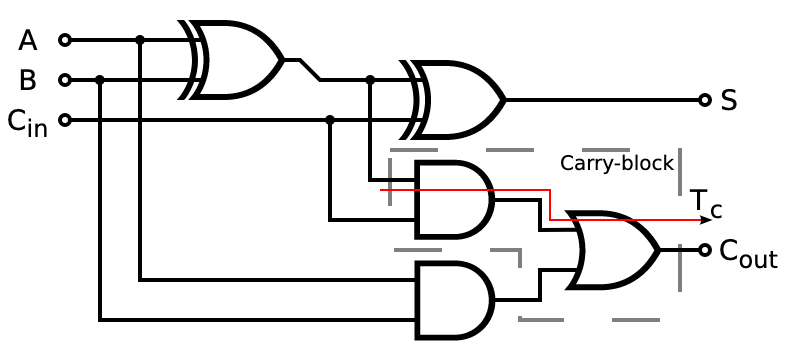
\includegraphics[width=\linewidth]{assets/full_adder_schematic.png}
    \centering
    \caption{
        Schematic of full adder implemented with two XOR gates, two AND gates,
        one OR gate.
    }
    \label{fig:full_adder_schematic}
\end{figure}

Instructions in machines are implemented using logical gates, such as AND, OR,
NOT and other gates. Logical gates are devices that perform boolean functions 
and are implementations of boolean formulae. In other words, we can model the
logical gates of the machine using boolean formulae \cite{page2009practical}.
The logical circuit of one instruction becomes a boolean formula in our model.
An example of a 1-bit full adder schematic can be seen in figure
\ref{fig:full_adder_schematic}. The schematic shows circuit logic for
arithmetic addition with two 1-bit inputs $A$ and $B$, one 1-bit value from
previous addition called carry in $C_{in}$ and it computes the 1-bit sum $S$
and 1-bit carry out $C_{out}$ value in case of an overflow. If we have a simple
RISC-V program containing the following series of instructions:
\begin{lstlisting}[language={[RISC-V]Assembler}, label=lst:example_riscv_program]
addi t0, zero, 4
addi t1, zero, 2
mul  t0, t0, t1
\end{lstlisting}
then we can model the program with the following operations:
\begin{lstlisting}[language=C, label=lst:example_model, caption=Example model, captionpos=b]
t0_1 = 0    + 4    && pc_1 = pc_0 + 4 &&
t1_1 = 0    + 2    && pc_2 = pc_1 + 4 &&
t0_2 = t0_1 * t1_1 && pc_3 = pc_2 + 4 
\end{lstlisting}

So the small RISC-V program can be reduced to the series of operations in
listing \ref{lst:example_model}. What we encoded is a satisfiability modulo
theory formula (SMT-Formula). That is, we encoded the program as a series of
operations in theory of bit-vectors. This model is satisfiable if and only if
there exists an assigment of values to variables such that the formula is true.
Variables in an SMT-Formula are bit-vectors and arrays of bit-vectors, hence
the theory of bit-vectors. Bit-vectors represent signed and unsigned integers
of arbitrary but fixed bit-length \cite{de2009satisfiability}, and bit vector
arrays which contain multiple values (either bit-vectors or arrays), indexable
by a bit-vector \cite{btor2}. Since the model we encoded operates on
bit-vectors and arrays of bit-vectors and not on boolean values, it is not
boolean logic. It is an intermediate step that must be further reduced to
boolean formula.

If we recall the full adder schematic in figure \ref{fig:full_adder_schematic},
we can see that the logic gates correspond to the following boolean formulae:

\begin{align*}
    S	    &= A \oplus B \oplus C_{in} \\
    C_{out} &= (A \land B) \lor (C_{in} \land (A \oplus B))
\end{align*}

This is a series of boolean formulae that describe the behaviour of the 1-bit
full adder. For two bit full adder, we would have two sum outputs $S_1, S_2$,
one initial carry in $C_{in1}$, and the carry out of the first sum $C_{out1}$
would be the carry in to the second sum $C_{out1} = C_{in2}$. The same process
applies for full adder of values with arbitrary bit length. The series of
operations in listing \ref{lst:example_model} can be encoded in a similar
way. This technique of encoding semantics of arithmetic and bitwise operations
is called bit-blasting \cite{barrett2021satisfiability}. We can add more
constraints to the model that do not come from the program, but rather specify
whether the machine reaches a particular state. For example, we can add
constraints that check whether a certain register of the machine (variable)
contains the value $0$ and we perform a division with that register. 

By doing so, we formulated a satisfiability problem, and by solving it we prove
that either our program does not perform division by zero for any given input,
or we get an example input for which the program performs division by zero. In
particular, by doing this, we reduced the state reachability problem to the
boolean satisfiability problem. Important observation is that the resulting 
boolean formula is finite and can model a finite number of executed
instructions, which makes our models bounded in the number of executed
instructions. This is the essence of bounded model checking.


\subsection{Complexity control with model parameters}

There are multiple possibilities when generating model and certain trade-offs
can be made. In our models of the machine, bit-vectors are used for values and
arrays of bit-vectors for main memory and registers. In particular, we used
one-dimensional arrays which contain bit-vectors of some fixed bit-length. When
modelling M-bit memory with an array that contains N-bit bit-vectors we need an
address space of $2^{(M - N)}$ entries. More precisely, the array must be
indexed with a bit-vector of bit length $(M - N)$. Size of bit-vectors stored
in the array represent the memory granularity - the size of each memory block
our machine can access. By changing the memory granularity we can directly
impact the size of the array.

When accessing memory each memory block is addressable by an address, which is
a bit-vector in our case. Logical circuit exists for this purpose in machine as
well. Naively implemented, this could be a chain of something similar to
if-else statements. In reality machines use a logical circuits such as
decoders, multiplexers and demultiplexers. Decoders have an N-bit address as
input which is decoded and used to activate one of $2^N$ possible outputs.
Multiplexer has $2^N$ inputs, one of which is selected based on the output
produced by the decoder given an N-bit address. Analog, demultiplexer has one
input which is routed to one of $2^N$ outputs based on the address
\cite{horowitz1989art}. Circuit logic of these components can be modelled as
boolean formulae as well, effectively modelling memory access of the machine.
Number of inputs for multiplexer (or outputs for demultiplexer) multiplied by
the size of each input is the size of modelled memory. The number of outputs of
address decoder must match the number of inputs/outputs of (de-)multiplexer.
Size of each input/output corresponds to memory granularity, and so the memory
granularity directly impacts the complexity of resulting circuit logic for
memory access and therefore the complexity of the model. Smaller memory
granularity requires more lines for input/output and larger memory addresses,
which increases complexity in all of the mentioned components.

\begin{figure}
    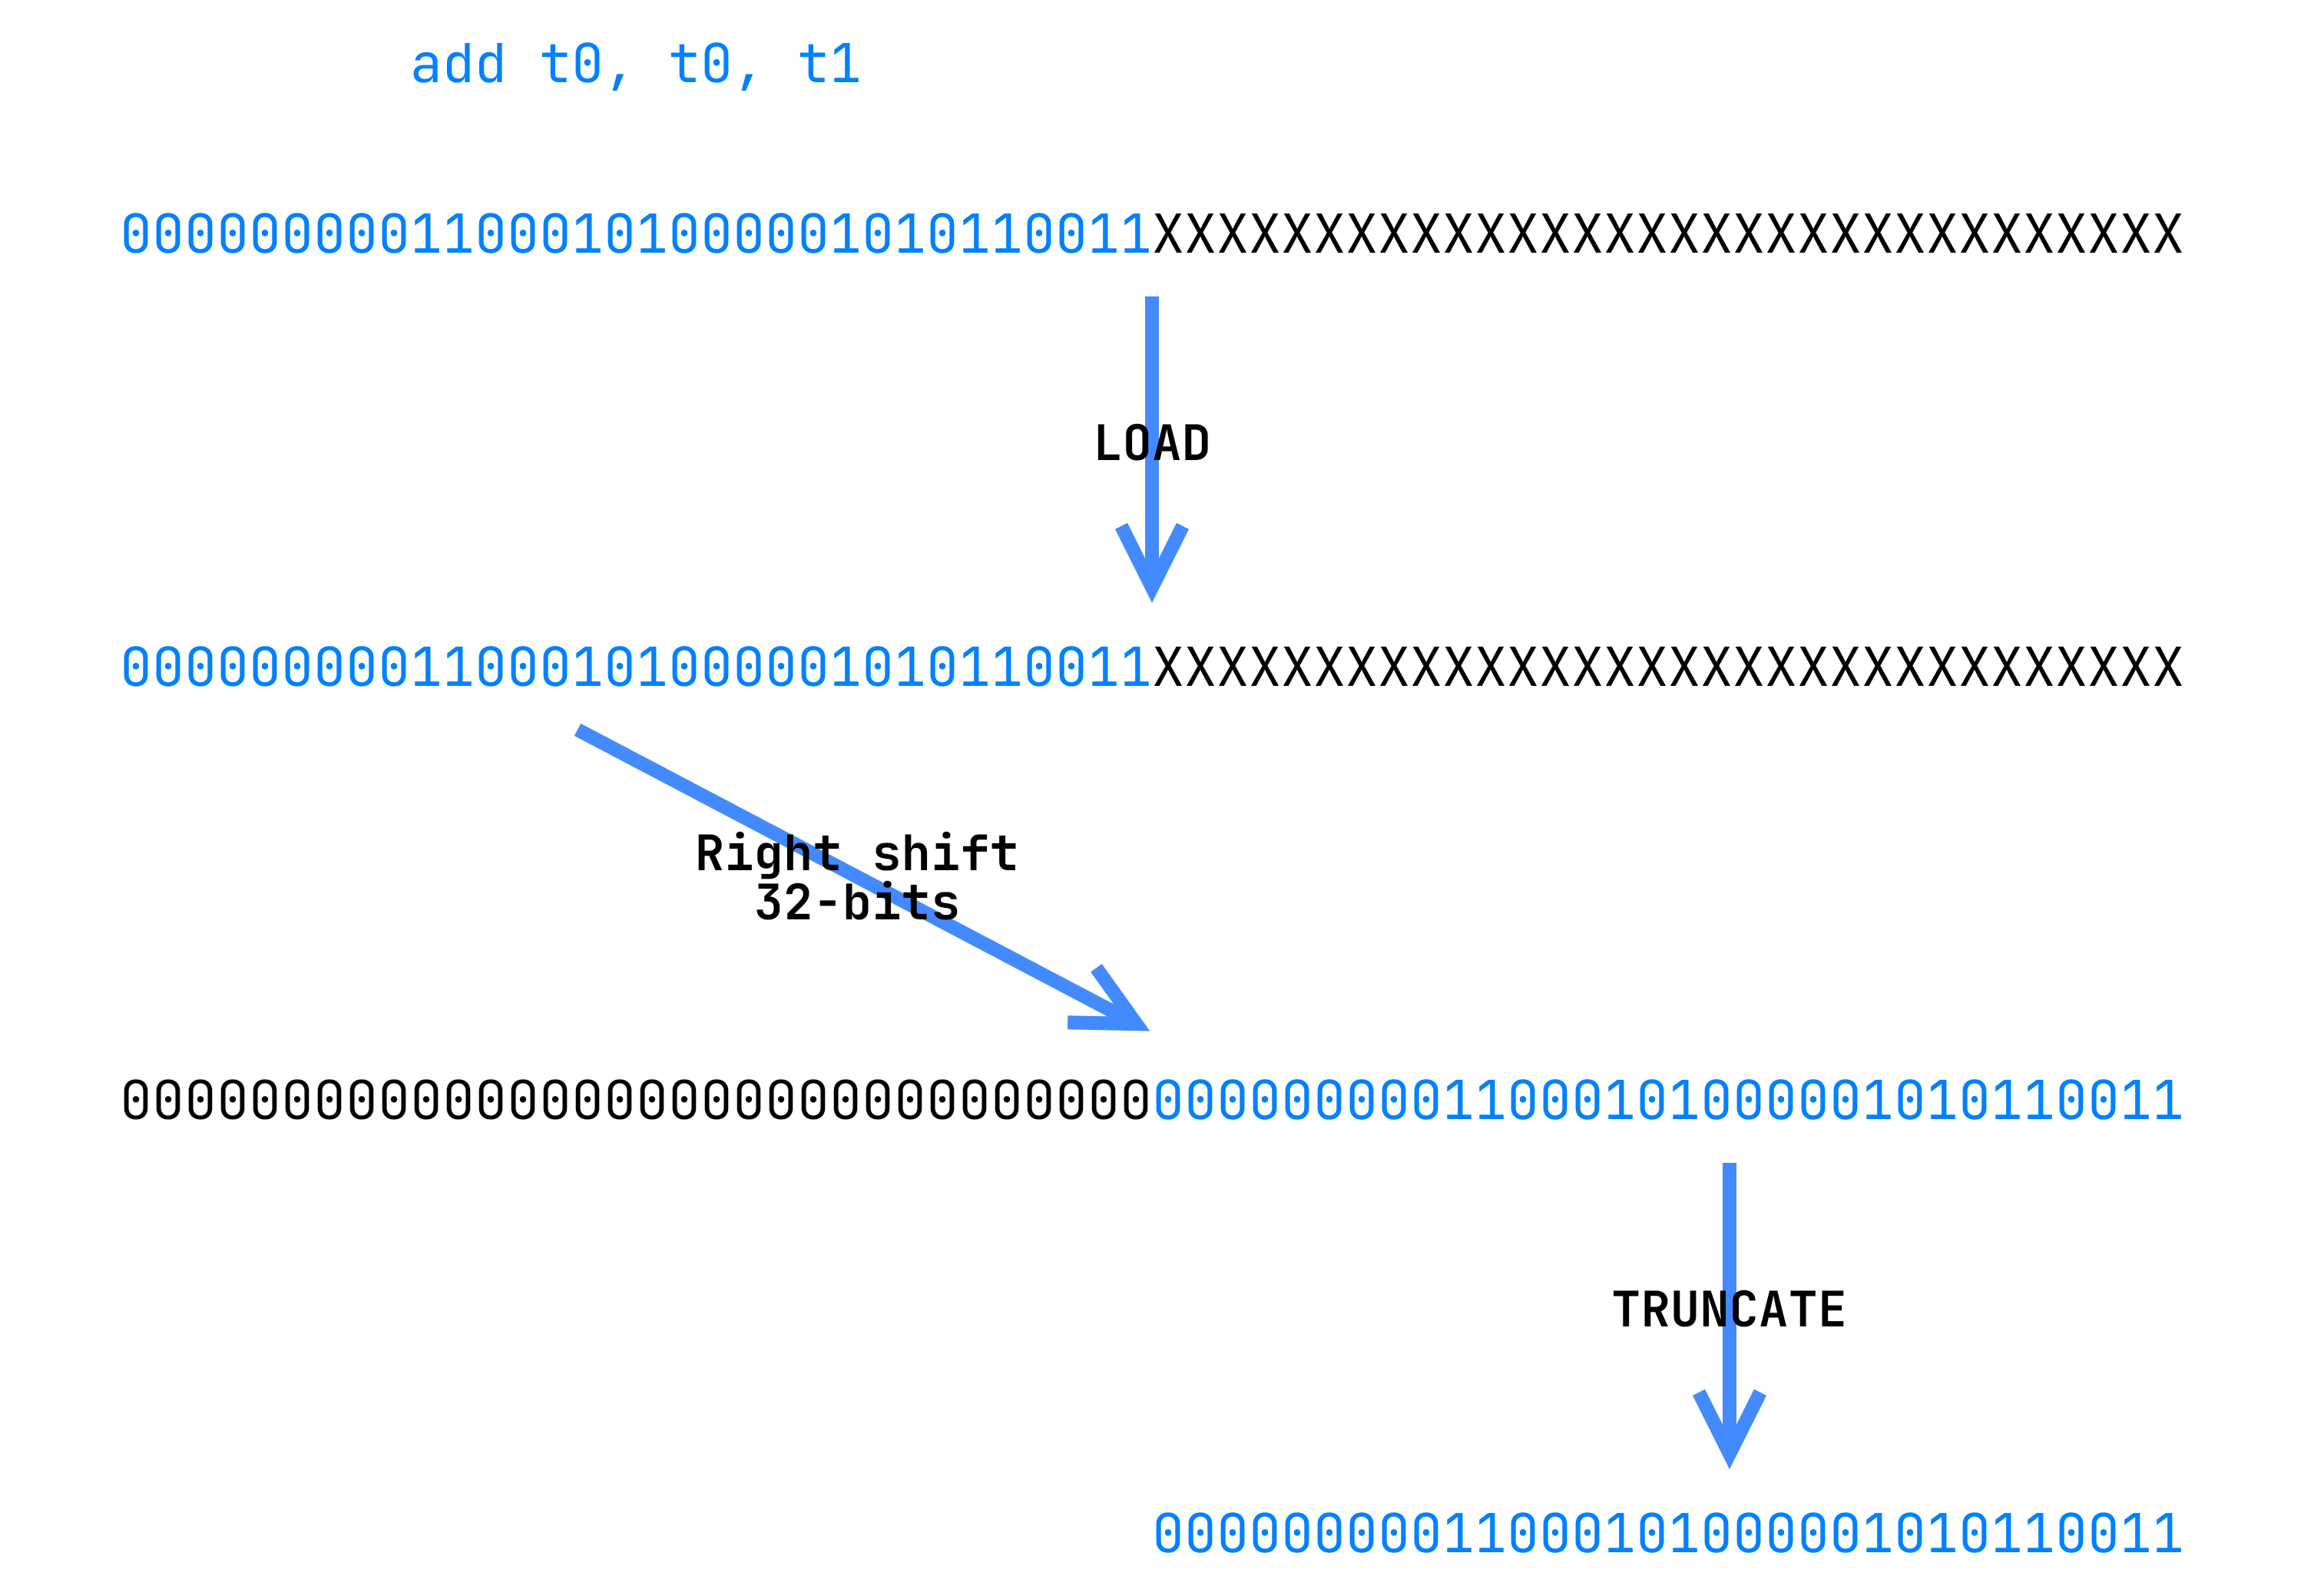
\includegraphics[width=\linewidth]{assets/64_bit_instruction_load.png}
    \centering
    \caption{Loading 32-bit instruction \cite{waterman2014risc} from memory with 64-bit granularity.}
    \label{fig:instruction_load_example}
\end{figure}

On the other hand, if we choose larger memory granularity, we can access the
whole memory with fewer addresses. Consequently, this reduces the complexity of
memory access circuits and therefore the complexity in corresponding part of
our model. However, it is not always the case that we need to access values in
memory that have the same size as our chosen granularity. When that's not the
case, we have to perform bit-shifting and bit-masking operations in order to
load the correct value. For example, if we want to load a 32-bit value from
memory with 8-bit granularity, we will have to access memory four times and
perform bit-shifting to store bits of value at the correct offset. Smaller
granularity in this case results in four memory accesses through large circuit
and four bit-shifting operations. If we, however, want to load a 32-bit value
from memory with 64-bit granularity, complexity varies greatly depending on the
alignment of the value in memory. As we can see in figure
\ref{fig:instruction_load_example}, when loading a value that is fully
contained inside of a 64-bit block, a single load with bit shifting and/or bit
masking will suffice. But if the value is split between two 64-bit blocks, we
need two loads, both bit shifting and bit masking and finally combining the two
values. Also, determining whether the value is split between two blocks
requires division operations to be performed, increasing the number of
operations on each access.

In our models, we can control the memory granularity and therefore influence
the complexity of models in various parts. In particular, we can control two
different parts of memory: memory that holds the program instructions (code)
and memory that holds the data (data, heap and stack segments). In particular,
we experimented with different combinations of code and data memory
granularity.


\section{Model generation}

In order to properly model the machine, we need to generate a model that
resembles it. Models need to precisely define the semantic of memory access and
machine instructions. As we already mentioned, we do not generate boolean
formula directly, but rather an SMT-Formula first. We use a special language
for this purpose called BTOR2.

\subsection{Introduction to BTOR2}

BTOR2 is an extension of BTOR, which is a format for quantifier-free formulae
over bit-vectors and arrays. BTOR2 extends BTOR by a set of additional features
and includes witness, invariant and fairness constraints and liveness
properties. BTOR2 supports defintion of sorts, which can be thought of as
types. For example, \texttt{sort bitvec 32} defines a sort of 32-bit
bit-vectors. Each line in BTOR2 format starts with an integer, which is either
a sort id for a sort definition, or node id for a node definition. Nodes in
BTOR2 can define operations such as addition, multiplication etc., or they can
be variable declaration, memory access, constraints and so on \cite{btor2}.

In listing \ref{lst:btor2_example} we can see an example of a model in BTOR2.
In first two lines we define two sorts, one is a 1-bit bit-vector with sort id
$1$, and the other is a 32-bit bit-vector with sort id $2$. In the following
line we have a node with node id $3$ that defines an input variable
\texttt{turn} of sort with sort id $1$, meaning that \texttt{turn} is a 1-bit
bit-vector. In the next line we define a constant $0$ of sort with sort id $2$.
In next two lines we define two 32-bit bit-vector state variables \texttt{a}
and \texttt{b}, and then initialize them with previously defined constant $0$.
We then define a constant $1$, which we use to increment the state variables.
We can observe that most of the keywords first reference a sort id. The
referenced sort id is the type of the node, and the node itself evaluates to a
certain value that we can reference by the node's id. In nodes $12$ and $13$,
we use an if-then-else construct, where we evaluate to a certain value based on
the condition. For state variable \texttt{a} we check whether the value of node
$3$ is $1$ ($true$), and if it is, the node $12$ evaluates to value of node
$5$, otherwise it evaluates to the value of node $10$. For state variable
\texttt{b} we check whether the value of node $3$ is false ($-3$ negates the
value of node $3$), and if so we use the value of node $6$, otherwise value of
node $11$. Since nodes $5$ and $6$ are definitions of state variables, using
them means using whatever the current value of the variable is. In nodes $14$
and $15$ we define the next function, which is the function that updates the
state variables, and these functions use the previously defined if-then-else
nodes for the update. In the next few lines we define a 32-bit bit-vector
constant $3$, we have two nodes that check whether our state variables have
value $3$. If both of them have value $3$, the node $19$ evaluates to $1$
(true), and in node $20$ we define a bad state. The node $20$ simply means, if
the value of node $19$ is $1$, then this bad state is reached. In listing
\ref{lst:c_code} we can see the corresponding \texttt{C} code for the BTOR2
model.

\begin{lstlisting}[label=lst:btor2_example, caption={Example BTOR2 model for \texttt{C} code in listing \ref{lst:c_code}},captionpos=b]
1 sort bitvec 1
2 sort bitvec 32
3 input 1 turn
4 zero 2
5 state 2 a
6 state 2 b
7 init 2 5 4
8 init 2 6 4
9 one 2
10 add 2 5 9
11 add 2 6 9
12 ite 2 3 5 10
13 ite 2 -3 6 11
14 next 2 5 12
15 next 2 6 13
16 constd 2 3
17 eq 1 5 16
18 eq 1 6 16
19 and 1 17 18
20 bad 19
\end{lstlisting}


\newpage
\begin{lstlisting}[label=lst:c_code, language=c, caption={\texttt{C} code we generate a model from},captionpos=b]
int main(void) {
    bool turn;
    unsigned int a = 0;
    unsigned int b = 0;

    while (1) {
        turn = read_bool();
        assert(!(a == 3 && b == 3));

        if (turn)
            a += 1;
        else
            b += 1;
    }
}
\end{lstlisting}

The BTOR2 format encodes the SMT-Formula. To solve the formula, we use a set of
tools that acompany the BTOR2 format available as part of the Boolector project
\cite{DBLP:journals/jsat/NiemetzPB14}. In particular, we use the reference
implementation of a bounded model checker \texttt{btormc}. The bit-blasting of
SMT-Formula is performed by the \texttt{btormc} before solving it. We run the
model checker by providing it the file containing BTOR2 model, and optionally
the upper bound. Upper bound option sets the maximal number of instructions
that can be checked. If the model checker terminates with no output, that means
that our program does not satisfy the given constraints in the number of
instructions we chose as the upper bound. On the other hand, if the program
satisfies the constraints, a witness format is produced. We can see an example
output of witness format in listing \ref{lst:btor_witness}.

\begin{lstlisting}[label=lst:btor_witness, caption={BTOR2 Witness Format for model in listing \ref{lst:btor2_example}}, captionpos=b]
sat
b0
@0
0 1 turn@0
@1
0 0 turn@1
@2
0 0 turn@2
@3
0 0 turn@3
@4
0 1 turn@4
@5
0 1 turn@5
@6
0 0 turn@6
.
\end{lstlisting}

The \texttt{sat} indicates that the model is satisfiable, \texttt{b0} is the 
satisfiable property with \texttt{b0} for 0-th bad property, that is the first
bad property that appears in the model. \texttt{@0} through \texttt{@6}
indicate the assignments of the inputs in frames 0 to 6, e.g., e.g., in frame
0 the 0-th input (first input defined in the BTOR2 model) \texttt{turn = 1} and
so on. Frame 6 is the last frame, where the bad property \texttt{b0} is
satisfied.

\subsection{\texttt{rotor} - tool of choice}

Generating BTOR2 models for programs is not done by hand. That would be tedious
and error prone, as models tend to be very large counting tens of thousands of
lines. Instead, we use a tool capable of generating BTOR2 models. Specifically,
we use \texttt{rotor}, which is a self-translating modeling engine based on
\texttt{selfie} that translates full RISC-V code including all of
\texttt{selfie} and itself to BTOR2 and SMT-LIB formulae that are satisfiable
if and only if there is input to the code such that the code exits with
non-zero exit codes, performs division by zero, or accesses memory outside of
memory segments. Rotor also generates models that enable RISC-V code synthesis
\cite{gh:rotor}.

\subsubsection{Model Parameters and Checks}

\texttt{rotor} accepts multiple arguments and parameters that can be used to
adjust produced models. By default multiple checks are enabled in
\texttt{rotor}, and we have to explicitely disable them using the following
command line arguments:

\begin{itemize}
    \item \texttt{-Pnobadexitcode} - Disables check for bad exit code. Without
        this option, the model checker will report satisfiable if the program
        can terminate with the chosen bad exit code.
    \item \texttt{-Pgoodexitcode} - Enables check for good exit code. With this
        enabled, the model is satisfiable if the program can exit with some 
        exit code other than the chosen good exit code.
    \item \texttt{-Pnoexitcodes} - Disables checking whether multiple cores
        exit with the same exit code. If not present, model is satisfiable if
        different cores can exit with different exit codes.
    \item \texttt{-Pnodivisionbyzero} - Disables division by zero check, which
        checks whether an input for the program exists such that the program
        performs division by zero.
    \item \texttt{-Pnodivisionoverflow} - Disables check for division (or
        remainder) overflow. Without this option, model is satisfiable if an
        input exists such that program performs division with an overflow.
    \item \texttt{-Pnosegfaults} - Disables check for segfaults, which checks
        whether the program accesses memory outside of defined memory segments.
\end{itemize}

Apart from these checks, we can also modify some parameters of the model.
Models generated for benchmarking in this thesis are generated with following
parameters: 

\begin{itemize}
    \item \texttt{-bytestoread 1} - Input of the program is 1 byte
    \item \texttt{-cores 1} - Machine has a single core
    \item \texttt{-virtualaddressspace 32} - 32-bit virtual address space
    \item \texttt{-codewordsize X} - Granularity of the code memory segment,
        where \texttt{X} is the size of the code memory segment in bits
    \item \texttt{-memorywordsize X} - Granularity of the non-code memory
        segments (data, stack and heap), where \texttt{X} is the size of the
        memory segment in bits.
    \item \texttt{-heapallowance 4096} - Maximum heap size in bytes
    \item \texttt{-stackallowance 4096} - Maximum stack size in bytes
\end{itemize}

As we can see, the memory granularity of code and non-code memory segments can
be independently configured. This was used to generate models with different
combinations of code and non-code memory granularity. We can generate many 
models rather quickly, because the generation of models is linear to the size
of the input program. \texttt{rotor} accepts either \texttt{C*} source code,
binary compiled by \texttt{starc} or binary compiled by \texttt{gcc} as inputs.
In case of using binaries as input, they must be compiled for the
\texttt{RISC-V} architecture.


\section{Experiment setup}

Running the experiment consists of multiple steps. This includes obtaining
binaries compiled for RISC-V architecture and generating models in BTOR2 format
from those binaries. After that, \texttt{btormc} is run on each model multiple
times, measuring and tracking the time it took to solve the model. We also want
to confirm that models are correct and are satisfiable for the right reason.
With the goal to facilitate this process, we introduce \texttt{peRISCope}.

\subsection{peRISCope}

\texttt{peRISCope} is a benchmarking toolbox designed to make the process of 
parameterized model generation and benchmarking of model solving easier
\cite{Fejzic_peRISCope}. The tool also supports parsing of BTOR2 witness format
in order to provide more information, such as which property was satisfied, and
transitions of inputs through frames that satisfy said property.
\texttt{peRISCope} accepts a configuration file in either \texttt{YAML} or
\texttt{JSON} format, which can be used to specify the parameters for models,
timeout for maximum duration of model solving, list of files for filtering, and
flags for \texttt{btormc}. The \texttt{peRISCope} performs multiple runs,
each time invoking \texttt{rotor} with parameters of that run which results in
multiple models being generated in a (specific) subdirectory inside
\texttt{selfie}. Model generation is fast, so we can generate models for all
example files without filtering. After the models are generated,
\texttt{btormc} is run on each model multiple times using \texttt{hyperfine}
\cite{Peter_hyperfine_2023}, measuring the time it took each time. In the
example configuration file shown in listing \ref{lst:periscope_config} we tell
the \texttt{peRISCope} to generate models with different code memory
granularity and to benchmark only models that match any of the entries in the
\texttt{files} list. The \texttt{timeout} parameter sets the maximum number of
seconds solving is allowed to take.

\begin{lstlisting}[label=lst:periscope_config, caption={Example peRISCope
                configuration file in \texttt{YAML} format}, captionpos=b]
timeout: 300
files:
  - "division-by-zero-3-35-rotorized.btor2"
  - "invalid-memory-access-fail-2-35-rotorized.btor2"

runs:
  8-bit-codeword-size: "0 -codewordsize 8"
  16-bit-codeword-size: "0 -codewordsize 16"
  32-bit-codeword-size: "0 -codewordsize 32"
  64-bit-codeword-size: "0 -codewordsize 64"
\end{lstlisting}

\subsection{Benchmarking Workflow}

The \texttt{peRISCope} can be compiled to a binary and at the time of this
writing supports two commands. One command is \texttt{parse-witness} which
takes witness format of \texttt{btormc} as input. The witness format is parsed,
and the flow of inputs and states through frames is printed to \texttt{stdout}
in a condensed format, as can be seen in listing \ref{periscope:parse_witness}.
This command has an optional parameter which is used to provide the path to
BTOR2 model file for which the witness format was generated. \texttt{peRISCope}
reads the BTOR2 file and extracts more information about the model such as the
names of properties that were satisfied. This enables \texttt{peRISCope} to
display additional information in the result of witness parsing and evaluation,
like in listing \ref{periscope:parse_witness_ctx}.

\begin{lstlisting}[label=periscope:parse_witness, caption={Example output of
                \texttt{peRISCope} \texttt{parse-witness} command.},
                captionpos=b]
Satisifed properties in 77 steps:
    Bad at 7

Inputs flow:
States flow:
    input-buffer:
           #0: 48 ([00000000] -> 00110000)
        -> #1: end
\end{lstlisting}

\begin{lstlisting}[label=periscope:parse_witness_ctx, caption={Example output
                of \texttt{peRISCope} \texttt{ parse-witness} command with
                provided BTOR2 file for context.}, captionpos=b]
Satisifed properties in 77 steps:
    Bad at 7 named 'core-0-division-by-zero' with nid: 37027

Inputs flow:
States flow:
    input-buffer:
           #0: 48 ([00000000] -> 00110000)
        -> #1: end
\end{lstlisting}

The output of \texttt{peRISCope} command \texttt{parse-witness} describes that
the given properties were satisfied in some number of frames. Additionally, it
shows that the \texttt{input-buffer} variable, modelled as \texttt{state} in
BTOR2, is assigned value $48$ at frame $0$, and it did not change until the
very last frame.

The second command of \texttt{peRISCope} is the \texttt{bench} command. This
command orchestrates the execution of multiple different commands. First, it 
runs the \texttt{rotor} generating models with specific configuration. Then it
runs \texttt{hyperfine} executing \texttt{btormc} on each model, collecting
benchmarking statistics. \texttt{btormc} may run very long for certain models,
so if the \texttt{timeout} option is set in the used configuration, we wrap the
invokation in the \texttt{timeout} command of GNU coreutils
\cite{gnu:coreutils}. We mark the result as \texttt{Failed} if we use
\texttt{timeout} and the model solving does not terminate within the specified
time. Otherwise, witness format is generated, parsed alongside the provided
BTOR2 model for context. The result of the whole run is then stored in a
results file, example of which can be seen in listing \ref{lst:results_file}.

The results are stored in \texttt{JSON} format, with one entry per BTOR2 model
file. The \texttt{Success} key indicates that \texttt{btormc} terminated, and
list of satisfied properties is presented. Further, we store the number of
frames it took to satisfy the properties and the results of \texttt{hyperfine}
benchmark runs, containing statistics as well as specific timings and exit
codes of each run. We also store the word count in BTOR2 model file, and also
word count of \texttt{btormc} dump for the same model file after it processed
it. This is useful for tracking the correlation between model size and the time
it took solving it.

Accompanying the \texttt{peRISCope} binary, we also have a script written in
Python. The script takes the results file as input and generates plots for
easier visual inspection of the results. The script supports different types of
plots, such as box plots and histograms. Linear and log scaling of plots are
available. Figure \ref{fig:results_plot} is one such plot.

\begin{figure}
    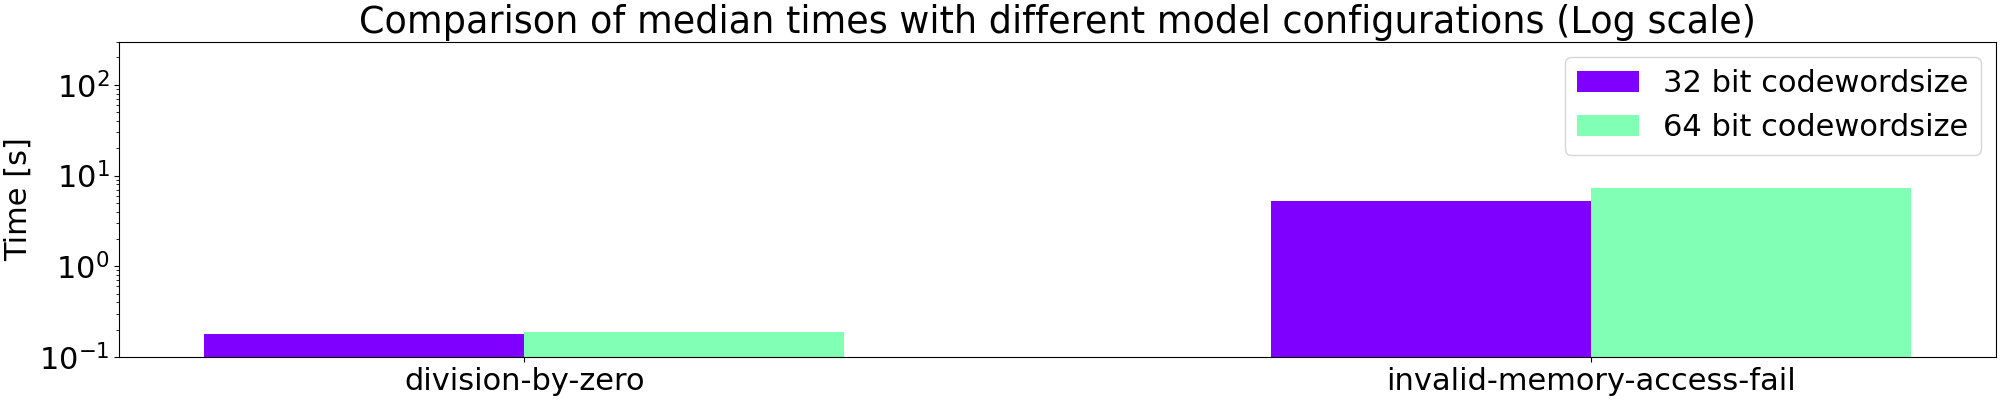
\includegraphics[width=\linewidth]{assets/plot_example.png}
    \centering
    \caption{
        Plot of results for two BTOR2 models with log scale.
    }
    \label{fig:results_plot}
\end{figure}

The models can be generated from \texttt{C*} source code. \texttt{rotor}
handles this by first compiling the source code with \texttt{starc} and then
generating the BTOR2 model from the resulting binary. The models can also be
generated from binaries directly. \texttt{rotor} has a flag \texttt{-l} for
loading a binary file. Binaries comiled with either \texttt{starc} or
\texttt{gcc} are supported. The \texttt{starc} compiles binaries for RISC-V
architecture out of the box. In case of \texttt{gcc} we either have to compile
the binaries on a RISC-V machine, or we have to use the RISC-V toolchain for
cross-compilation \cite{riscv_gnu}. In this thesis, we compiled binaries and
generated models from the same set of \texttt{C*} source code files with both
\texttt{starc} and \texttt{gcc}. In particular, we used the files found in
\texttt{examples/symbolic/} directory in the \texttt{selfie} repository
\cite{gh:rotor}.

The benchmarks were run on a machine with following specifications: 
\begin{itemize}
    \item Huawei Matebook 16 (model: CREM-WFD9)
    \item CPU: AMD Ryzen 7 5800H (16-core) clocked at 4.46 GHz
    \item Graphics: AMD Radeon Vega Mobile Series (Integrated)
    \item Memory: 16GB LPDDR4-4167
\end{itemize}
\newpage
\begin{lstlisting}[label=lst:results_file, caption={Example of \texttt{peRISCope} results file}, captionpos=b]
{
  "division-by-zero-3-35-rotorized.btor2": {
    "Success": {
      "props": [
        {
          "kind": "Bad",
          "name": "core-0-division-by-zero",
          "node": 37027,
          "idx": 7
        }
      ],
      "steps": 77,
      "hyperfine": {
        "results": [
          {
            "command": "btormc division-by-zero-3-35-rotorized.btor2 -kmax 200",
            "mean": 0.3718056574400001,
            "stddev": 0.008814608910627868,
            "median": 0.37023892844,
            "user": 0.33166193999999993,
            "system": 0.0399969,
            "min": 0.36236449744,
            "max": 0.38613962244,
            "times": [
              0.37023892844,
              // ...
            ],
            "exit_codes": [
              0,
              // ...
            ]
          }
        ]
      },
      "wc_raw": 273051,
      "wc_btormc_dump": 93238
    }
  }
}
\end{lstlisting}
\newpage

\section{Experiment results}

With the setup described in previous section, we generated BTOR2 models with 
following examples: 

\begin{itemize}

    \item Simple assignment - satisfiable on specific input manipulated with
        basic arithmetic.

    \item Division by zero - satisfiable if division by zero is performed.

    \item Invalid memory access fail - satisfiable if invalid memory is
        accessed, such as memory at an address outside of the virtual address
        space.
    \item Memory access fail - satisfiable if bad memory access is performed,
        such as unaligned memory access.

    \item Simple if without else - satisfiable when the input satisfies the
        condition of an if statement without an else block.
    \item Simple if-else - satisfiable when the input satisfies the condition
        of an if statement.
    \item Simple if-else reverse - satisfiable if the input does not satisfy
        condition of an if statement so that the body of the \texttt{else}
        block is executed.

    \item Nested if-else - satisfiable when body of an if statement inside of
        another if statement is executed.
    \item Nested if-else reverse - satisfiable when body of an if statement
        inside of an else block is executed.

    \item Recursive ackermann - satisfiable if ackermann function is computed
        with a specific input.
    \item Recursive fibonacci - satisfiable if fibonacci function is computed
        with a specific input.
    \item Recursive factorial fail - satisfiable if factorial function is
        computed with a specific input.
    \item Nested recursion fail - satisfiable if nested recursion is performed
        with a specific input.

    \item Return from loop - satisfiable if a loop exits with a return
        statement, which happens with digit as the input.
    \item Simple increasing loop - satisfiable if a loop is run exact number of
        times, depending on the input value used in the loop condition which is
        incremented in each iteration.
    \item Simple decreasing loop - satisfiable if a loop is run exact number of
        times, depending on the input value used in the loop condition which is
        decremented in each iteration. 
    \item Three level nested loop fail - satisfiable if three nested loops that
        use input in their condition run specific number of times.
    \item Two level nested loop - satisfiable if two nested loops that use
        input in their condition run specific number of times.

\end{itemize}

Each of the examples is contained in separate source code file. We compiled
each of the files both with \texttt{starc} and \texttt{gcc} compilers, and
generated BTOR2 models with different combinations of code-word and memory-word
sizes. The benchmark results of bounded model checking (with 200 as the upper
bound) for each model are presented in the following two sections.

\subsection{Results with binaries compiled with selfie}

\begin{figure}[!h]
    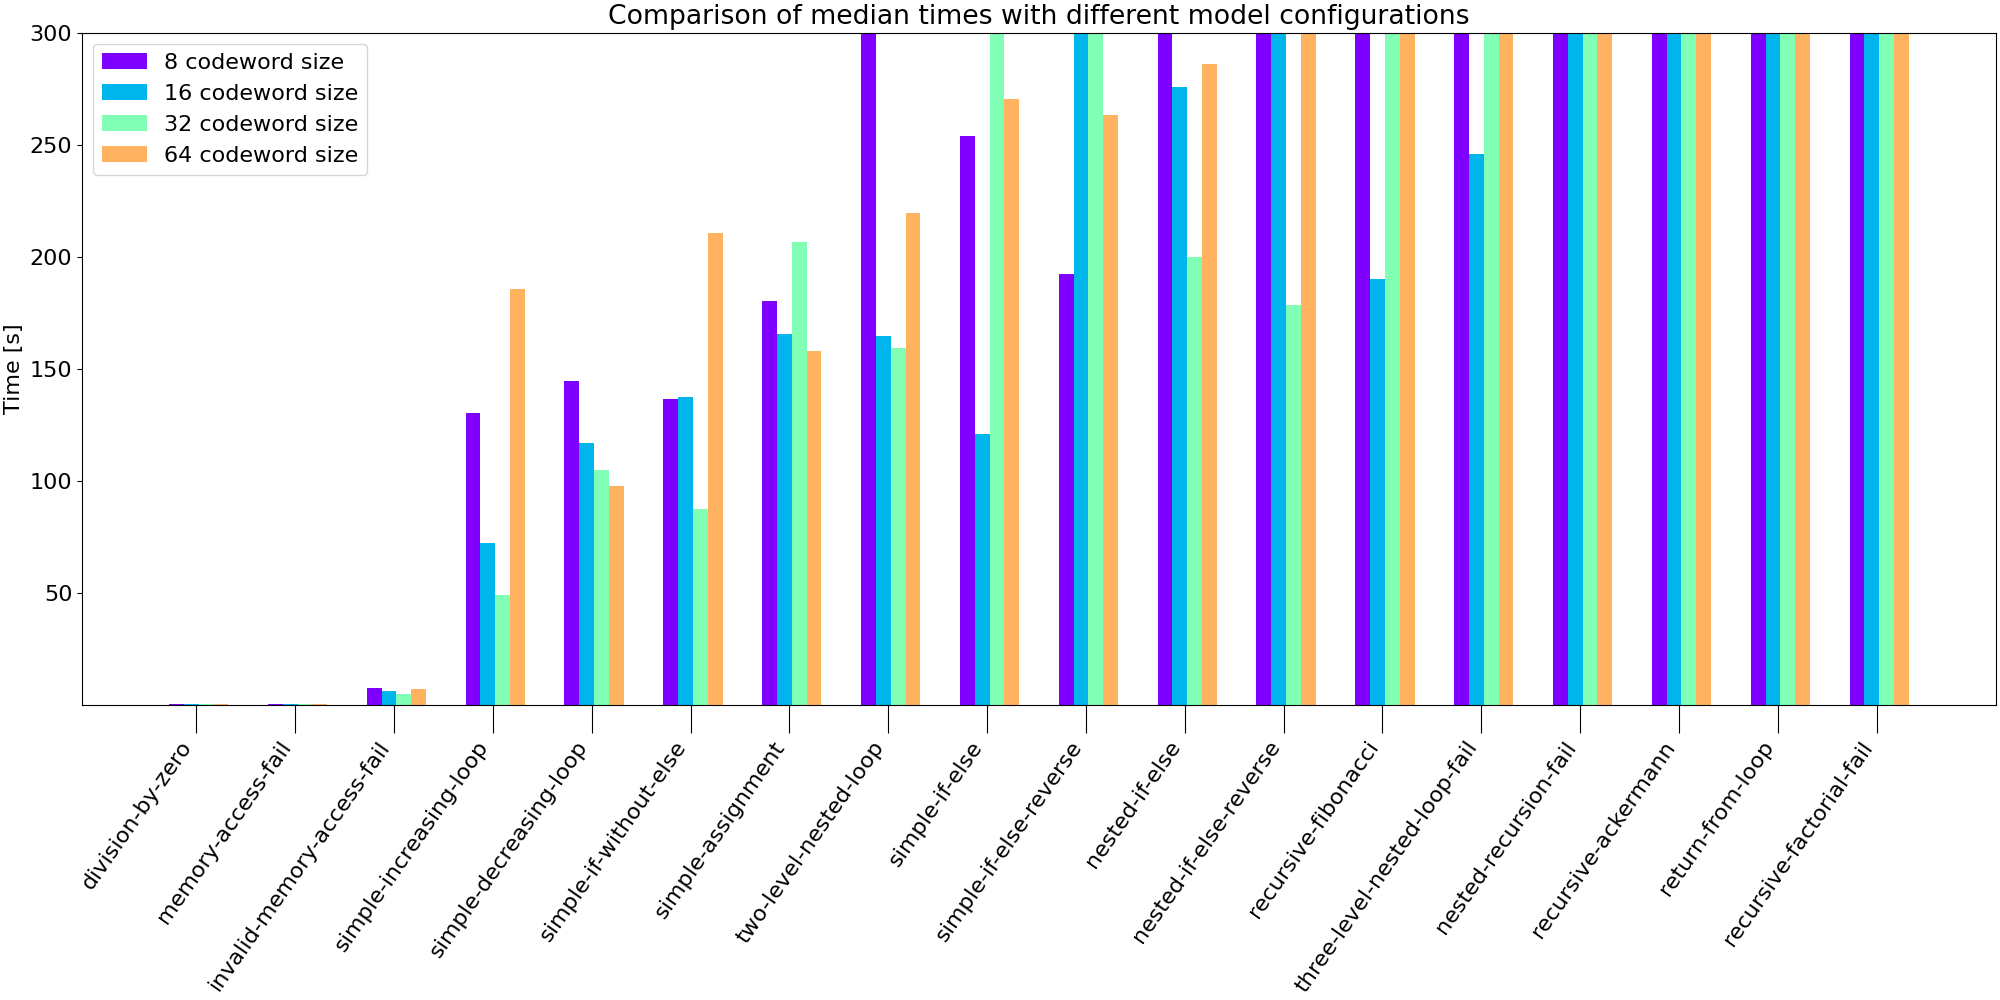
\includegraphics[width=\linewidth]{assets/benches/codeword_selfie_linear.png}
    \centering
    \caption{
        Selfie compiled binaries - codeword size comparison
    }
    \label{fig:codeword_selfie_linear}
\end{figure}

\begin{figure}[!h]
    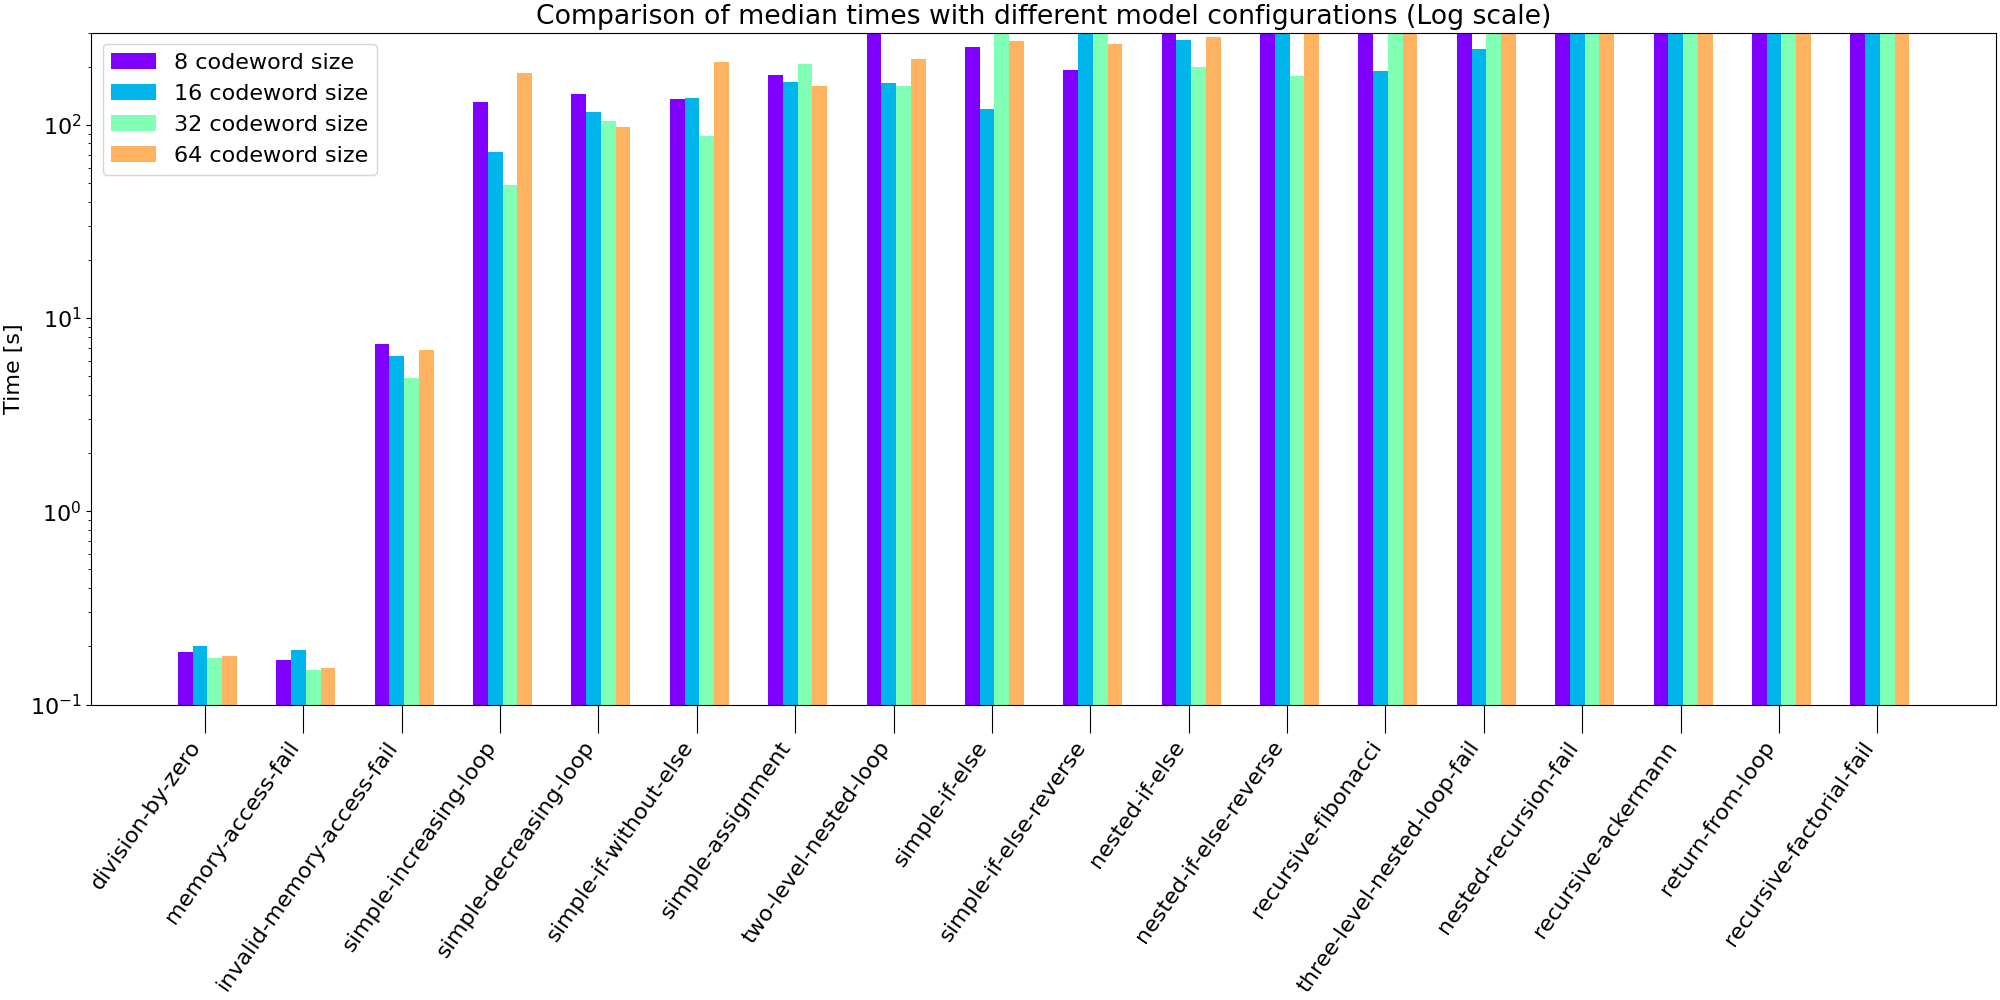
\includegraphics[width=\linewidth]{assets/benches/codeword_selfie_log.png}
    \centering
    \caption{
        Selfie compiled binaries - codeword size comparison (Log scale)
    }
    \label{fig:codeword_selfie_log}
\end{figure}

The time it took to solve BTOR2 models generated from binaries compiled with
\texttt{starc} compiler in \texttt{selfie} are presented in figures
\ref{fig:codeword_selfie_linear} and \ref{fig:codeword_selfie_log}. The solving
terminated within 300 seconds for 9 models configured with code-word size of
8-bits. In case of models with 32-bit code-word size, solving terminated for 10
such models, and for 11 models with 64-bit code-word size. As for the
configuration with 16-bit code-word size, solving terminated within 300 seconds
for 12 models. This configuration terminated approximately in the average
duration of all other models. However, solving terminated for more models with
this configuration than with any other. This indicates that time complexity
grows slower for models with 16-bit code-word size generated from
\texttt{starc} compiled binaries. This is somewhat surprising, as
\texttt{starc} compiled binaries contain only 32-bit RISC-V instructions.

\begin{figure}[!h]
    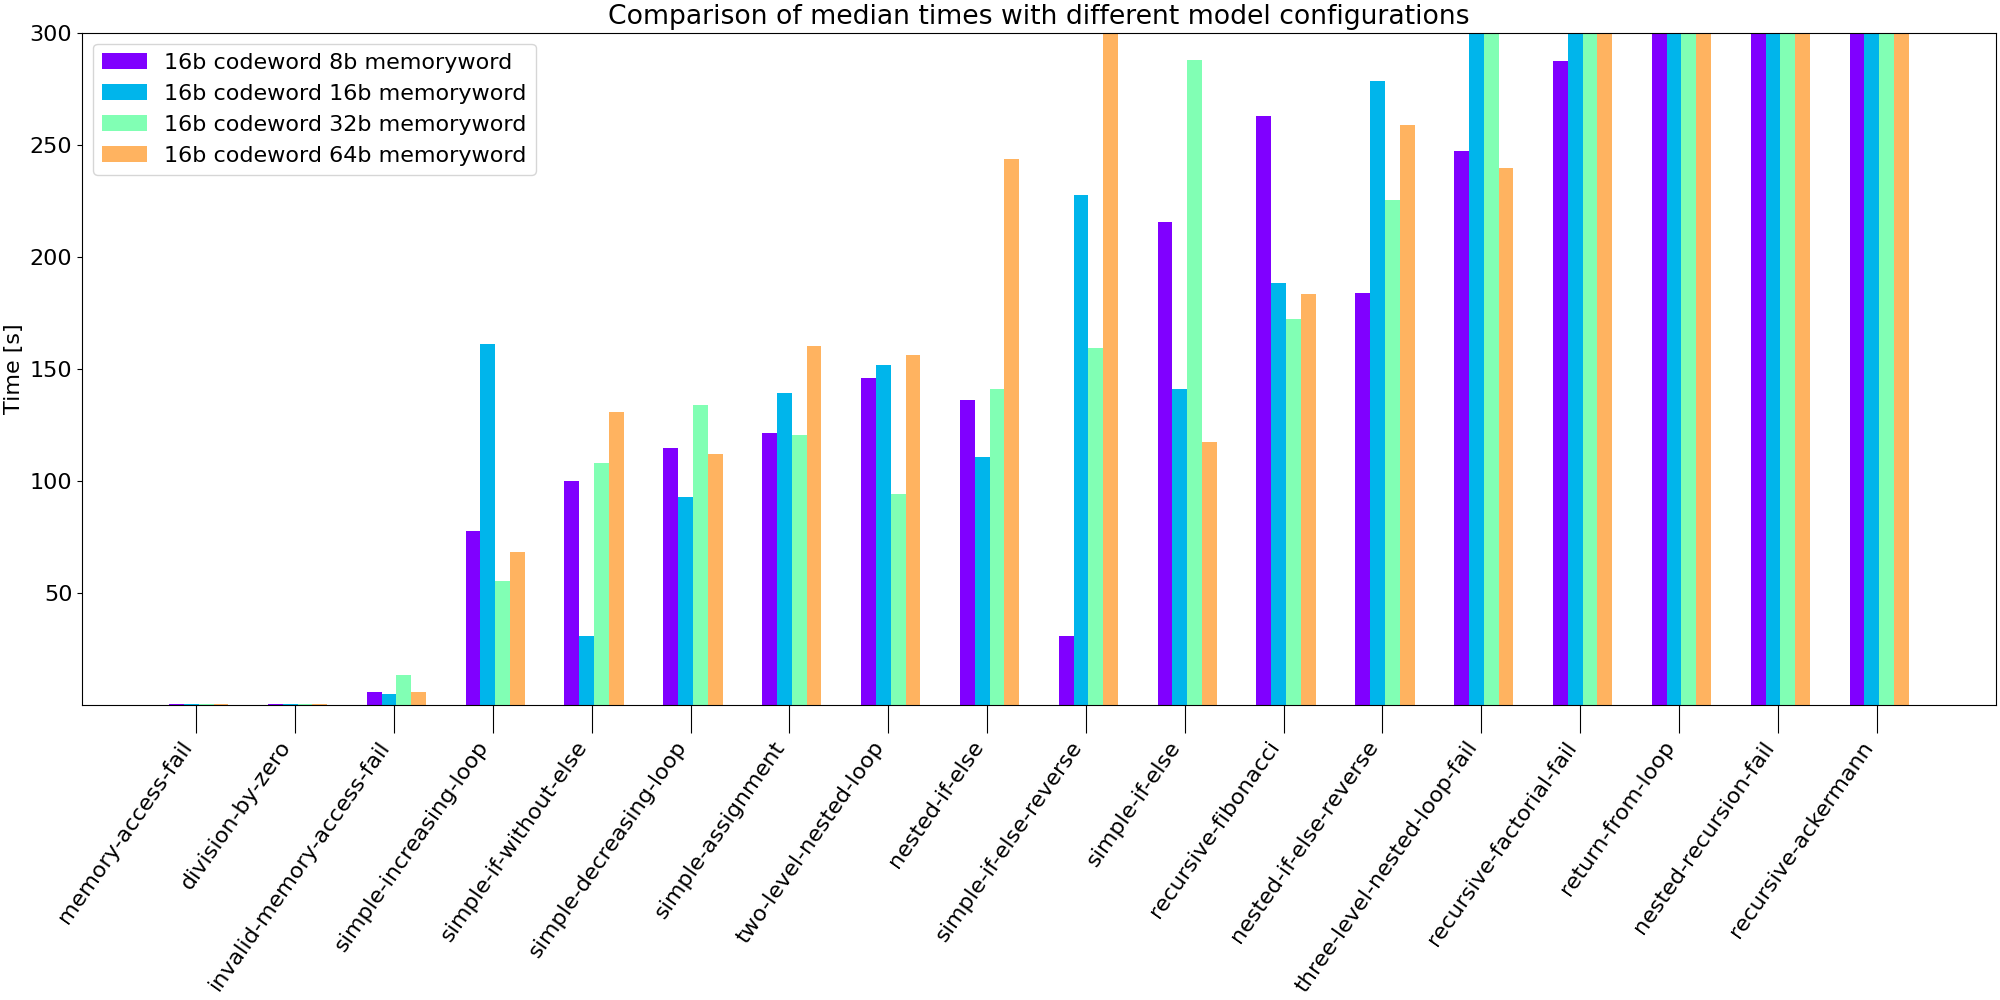
\includegraphics[width=\linewidth]{assets/benches/16b_codeword_memword_selfie_linear.png}
    \centering
    \caption{
        Selfie compiled binaries - fixed 16-bit codeword with varying memory word size comparison
    }
    \label{fig:16b_codeword_memword_selfie_linear}
\end{figure}

\begin{figure}[!h]
    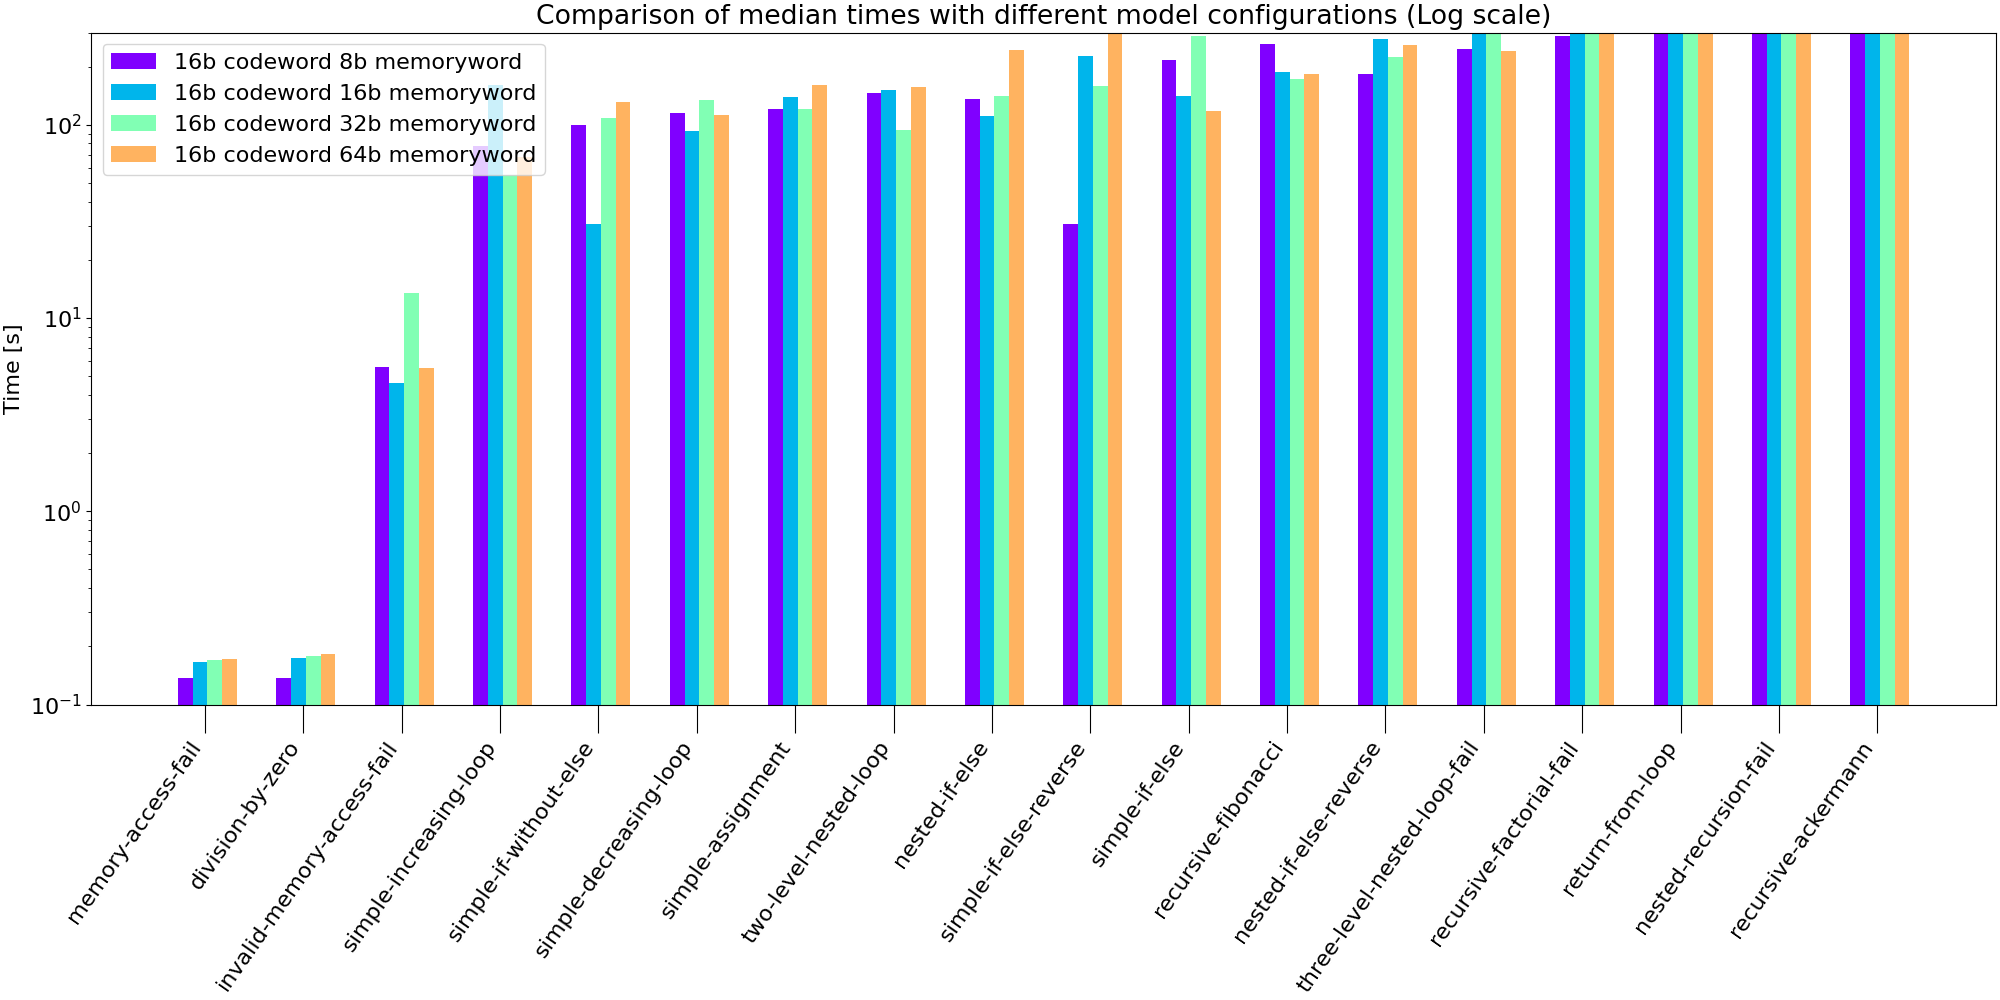
\includegraphics[width=\linewidth]{assets/benches/16b_codeword_memword_selfie_log.png}
    \centering
    \caption{
        Selfie compiled binaries - fixed 16-bit codeword with varying memory word size comparison (Log scale)
    }
    \label{fig:16b_codeword_memword_selfie_log}
\end{figure}

We proceeded with the 16-bit code-word size configuration, and generated models
with varying memory-word sizes. Comparison of solving time for these models in
figures \ref{fig:16b_codeword_memword_selfie_linear} and
\ref{fig:16b_codeword_memword_selfie_log} show that the configuration with
8-bit memory-word size terminated within 300 seconds for 15 models, 16-bit
memory-word size for 13 models, 32-bit memory-word as well as 64-bit
memory-word size configurations terminated for 13 models. The configuration
with 8-bit memory-word size was solved in shortest amount of time for 6 models.
16-bit memory-word size configuration was solved in shortest amount of time for
4 models, 32-bit memory-word size configuration for 3 models and 64-bit
memory-word size configuration for 2 models. Overall models generated from
\texttt{starc}-compiled binaries with smaller memory granularity configurations
terminated in shorter amount of tims.

\subsection{Results with binaries compiled with gcc}

The times it took for \texttt{btormc} to terminate for models with different 
codeword-size configurations from binaries compiled with \texttt{gcc} are 
presented in figures \ref{fig:codeword_gcc_linear} and
\ref{fig:codeword_gcc_log}. The \texttt{btormc} terminated within 300 seconds
for roughly half of the generated models. This was expected, because the models
generated from binaries compiled with \texttt{gcc} are much bigger. The results
can be better analyzed in the figure \ref{fig:codeword_gcc_log} with
logarithmically scaled time axis. Relations between 8-bit and 16-bit codeword
size configurations are similar to those between 32-bit and 64-bit codeword
size. The models with 8-bit codeword size configurations were solved faster
than those with 16-bit configurations in all but two cases. Similarly for
32-bit and 64-bit codeword size configurations. However, in those cases where
the models with smaller codeword memory granularity were solved faster, the
difference in time is insignificant, approximately half of a second. But in
cases where models with larger codeword size were solved faster, the time
difference is bigger, around a second between 64-bit and 32-bit configurations
and around 30-40 seconds between 16-bit and 8-bit configurations. Overall, the
shortest time it took to solve the models was for configurations with 64-bit
codeword size.

\begin{figure}
    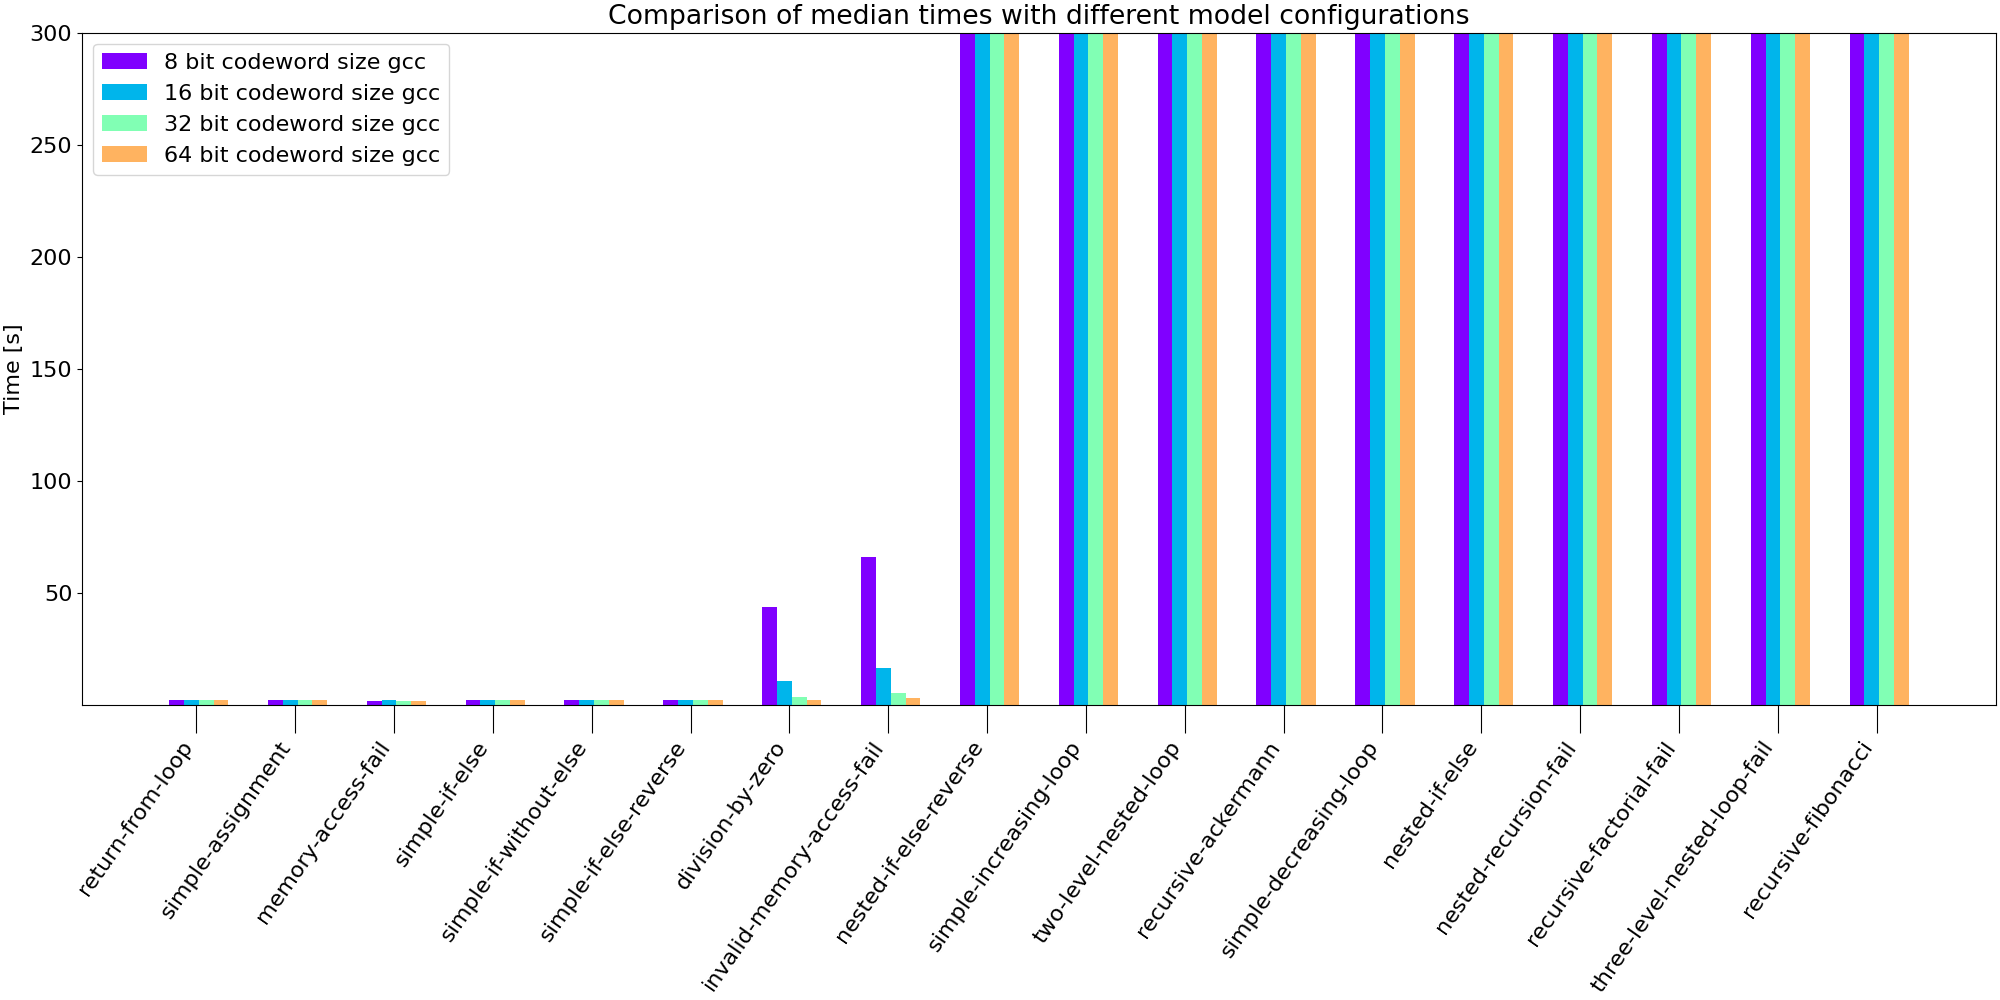
\includegraphics[width=\linewidth]{assets/benches/codeword_gcc_linear.png}
    \centering
    \caption{
        \texttt{gcc} compiled binaries - codeword size comparison
    }
    \label{fig:codeword_gcc_linear}
\end{figure}

\begin{figure}
    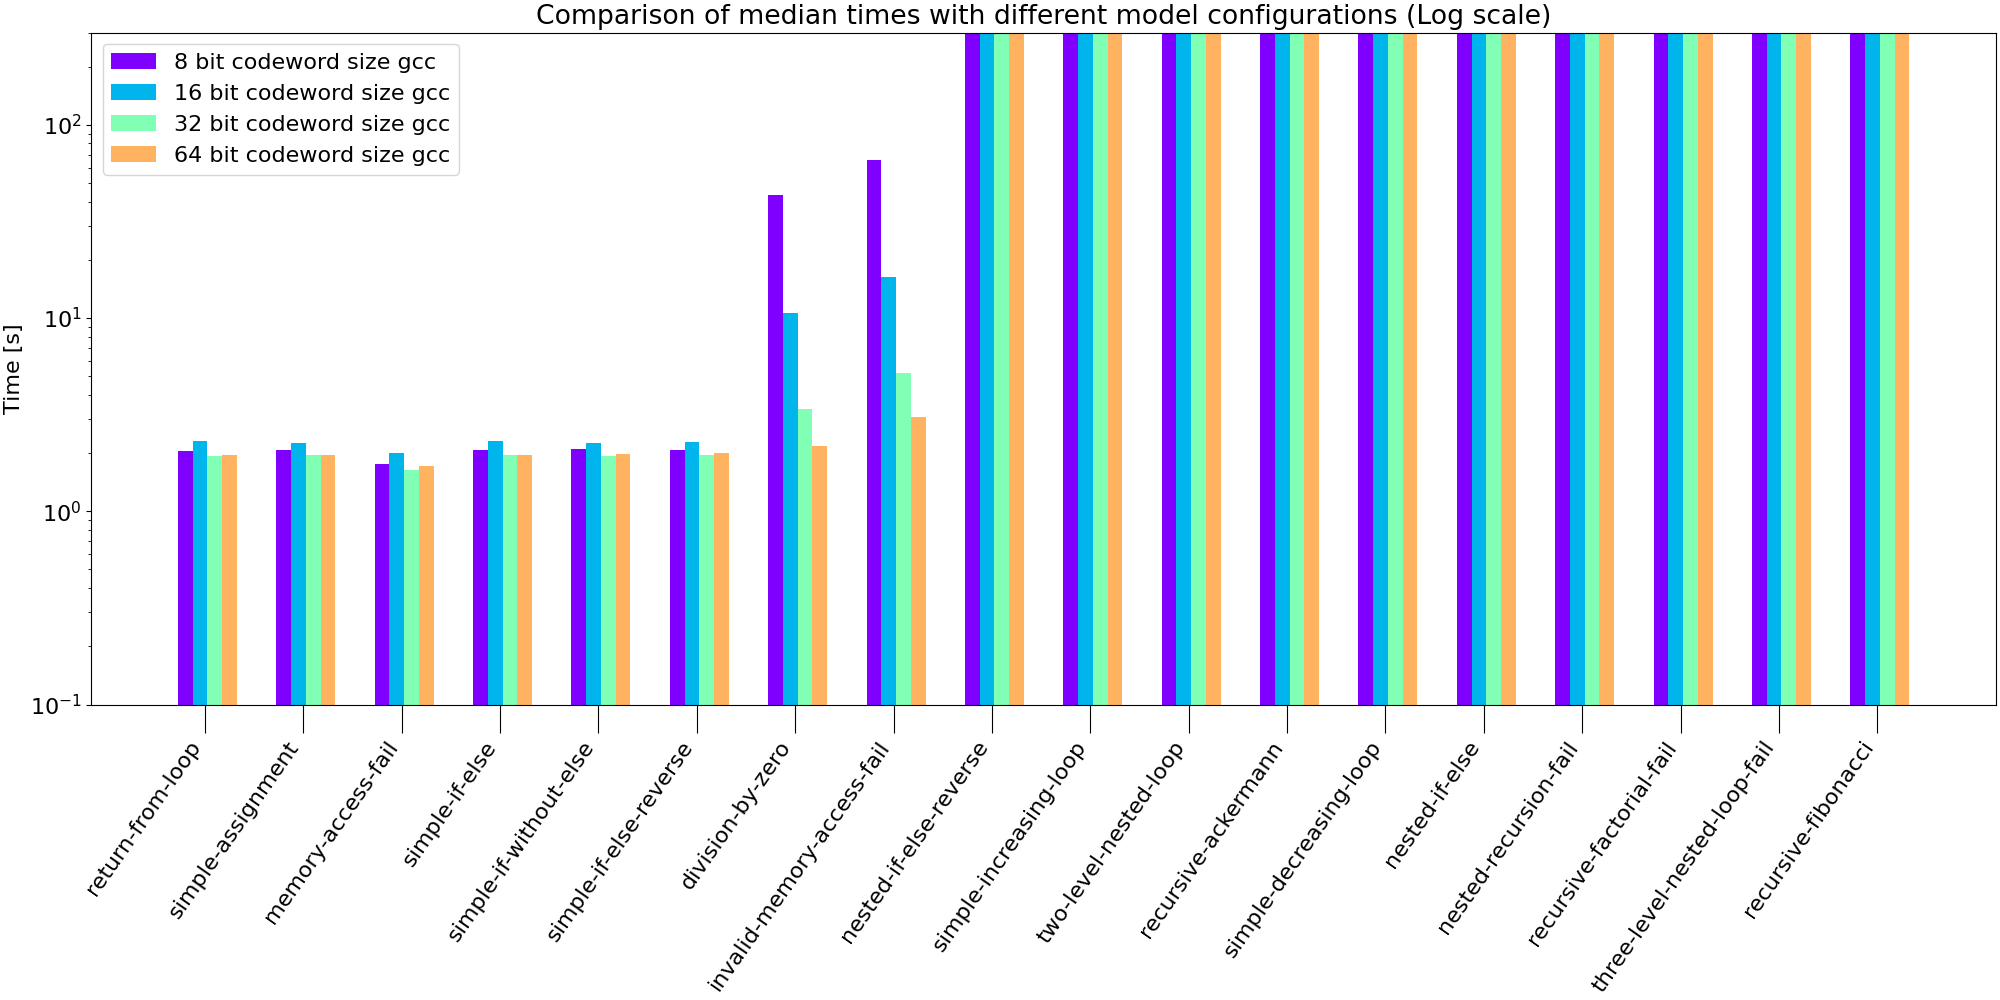
\includegraphics[width=\linewidth]{assets/benches/codeword_gcc_log.png}
    \centering
    \caption{
        \texttt{gcc} compiled binaries - codeword size comparison (Log scale)
    }
    \label{fig:codeword_gcc_log}
\end{figure}

\begin{figure}
    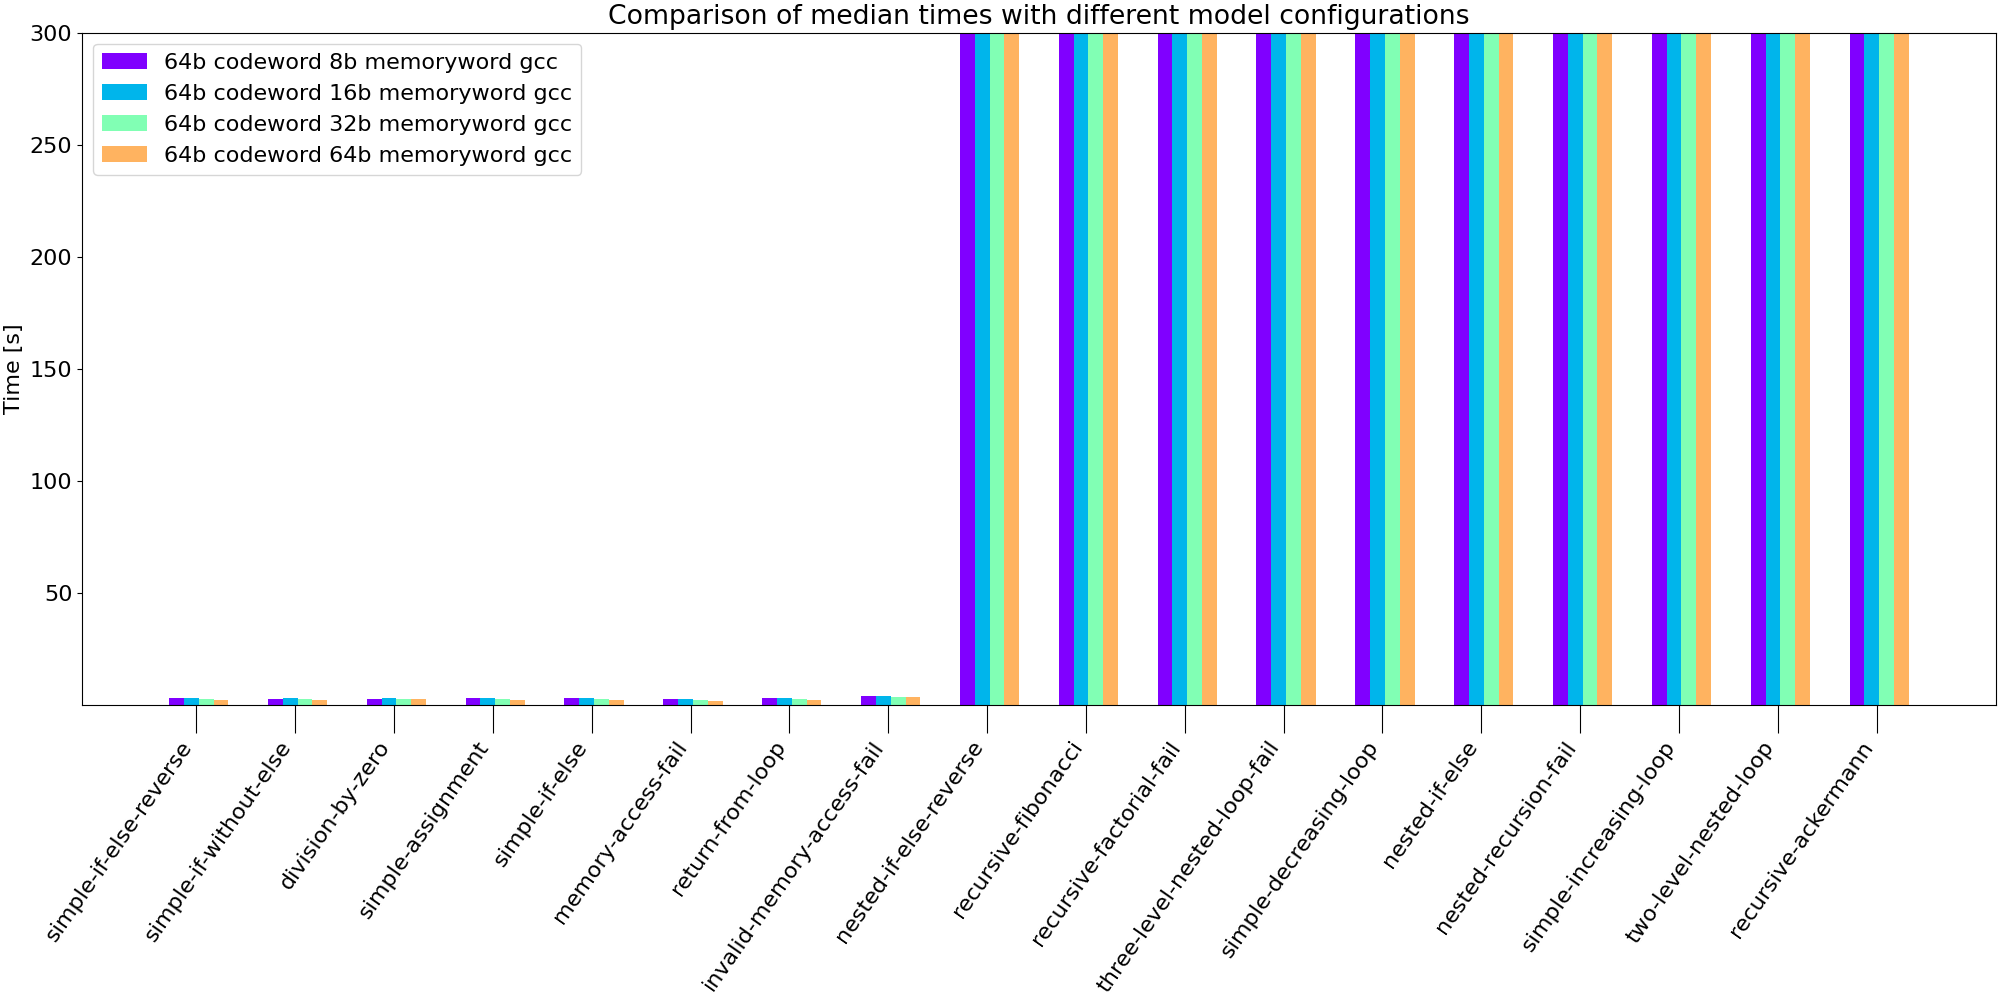
\includegraphics[width=\linewidth]{assets/benches/64b_codeword_memword_gcc_linear.png}
    \centering
    \caption{
        \texttt{gcc} compiled binaries - fixed 64-bit codeword, varying memory
        word size comparison
    }
    \label{fig:64b_codeword_memword_gcc_linear}
\end{figure}

\begin{figure}
    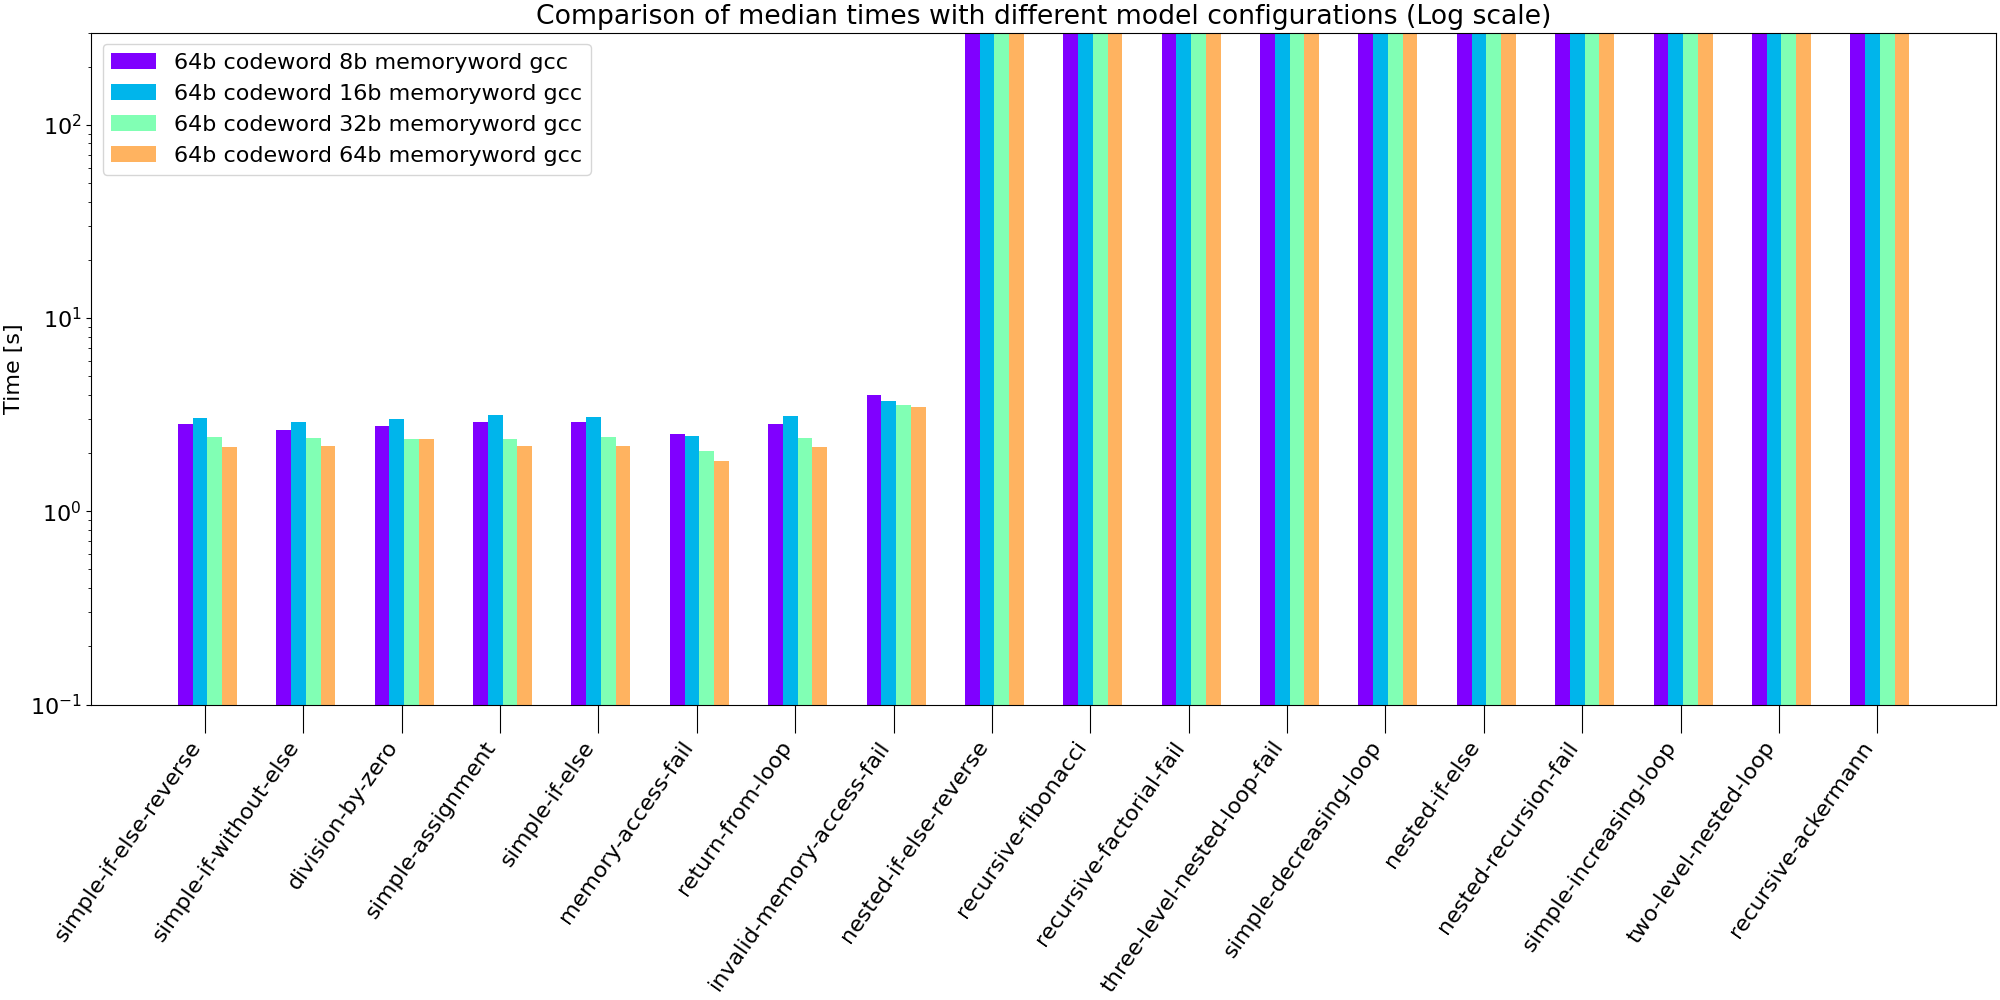
\includegraphics[width=\linewidth]{assets/benches/64b_codeword_memword_gcc_log.png}
    \centering
    \caption{
        \texttt{gcc} compiled binaries - fixed 64-bit codeword, varying memory
        word size comparison (Log scale)
    }
    \label{fig:64b_codeword_memword_gcc_log}
\end{figure}

As the models with 64-bit codeword size configuration were the ones that were
overall solved the fastest, we proceeded with this configuration, generated
models with varying memory-word sizes and obtained results shown in figures
\ref{fig:64b_codeword_memword_gcc_linear} and
\ref{fig:64b_codeword_memword_gcc_log}. \texttt{btormc} terminated for the same
number of models. We can clearly see that the models configured with 64-bits
for both codeword and memoryword sizes were solved in the shortest amount of
time. The models with 32-bit memory-word size come closely in second place. In
case of 8-bit and 16-bit memory-word size configurations, 8-bit configuration
was solved faster in all but 2 cases. Overall, we observe that in case of
\texttt{gcc} compiled binaries larger memory granularity seems to be more
beneficial.

\section{Conclusion and further work}

In this thesis, we discussed the importance and proving of program correctness.
We explained shortly, how to model the problem of proving correctness by
reducing the state reachability problem to the boolean satisfiability problem.
We showed how to generate SMT-Formula from a program, and then further reduce
it to a boolean formula by bit-blasting. Two new tools were presented,
\texttt{rotor} used for BTOR2 model generation, and \texttt{peRISCope} for
benchmarking orchestration of bounded model checking of generated models.
Finally, we ran the BTOR Model Checker \texttt{btormc}, measured the time it
took to solve the models generated from binaries compiled with \texttt{starc}
and \texttt{gcc}, and briefly discussed the results we observed. The results
indicate that solving of models generated from binaries compiled by
\texttt{starc} is faster for configurations with smaller code and non-code
memory granularity. In case of \texttt{gcc} compiled binaries, solving was
faster for models with largest code and non-code memory granularity. This might
be due to multiple reasons, such as the size of models, but also potential
optimizations implemented by \texttt{gcc} for 64-bit RISC-V architecture.
Future experiments could investigate the correlation between compiler
optimizations and the solving time.

The generated model configurations are not exhaustive. \texttt{rotor} supports
more options, such as specifying the number of cores, how many bytes of input
should be read and so on, and it can be extended to support even more options.
More exhaustive benchmarking of every possible combination would provide more
insight into the reasoning performance of RISC-V Software Models in BTOR2.

% \bigskip

%---------------------------------------------------------------------------------------------------------------------------------------
%---------------------------------------------------------------------------------------------------------------------------------------
%---------------------------------------------------------------------------------------------------------------------------------------

\newpage

\printbibliography

\newpage

%\topskip0pt
\vspace*{\fill}
\begin{center}
    \textbf{\Huge Statement of Authentication}\\
\end{center}

\vspace{1cm}

I hereby declare that I have written the present thesis independently, without
assistance from external parties and without use of other resources than those
indicated. The ideas taken directly or indirectly from external sources
(including electronic sources) are duly acknowledged in the text. The material,
either in full or in part, has not been previously submitted for grading at
this or any other academic institution.\\

\vspace{1cm}

Salzburg,\today \hspace{0.5cm}\hrulefill\\
\vspace{-0.5cm}
\flushright Nadir Fejzić

\vspace*{\fill}
\end{document}
